\documentclass[12pt,a4paper]{report}
\usepackage{config}

\pagestyle{main}

%%%%%%%%%%%%%%%%%%%%%%%%%%%%%%%%%%%%%%%%%%%%%%%%%%%%%%%

\begin{document}

% ===== HALAMAN SAMPUL =====
\thispagestyle{empty}
\newgeometry{margin=0cm}
\begin{tikzpicture}[remember picture, overlay]
    % --- Top accent bar ---
    \fill[accentdark] (current page.north west) rectangle
        ([yshift=-3.5cm]current page.north east);
    % --- Logo ---
    \node[anchor=center] at ([yshift=-1.75cm]current page.north)
        {
\includegraphics[scale=0.15]{Figure/ifitera-header.png}};
\end{tikzpicture}
\begin{center}
    \vspace*{4.5cm}
    {\color{textsec}\large\MakeUppercase{\textls[120]{Modul Praktikum}}}\\[0.6cm]
    {\color{accentdark}\fontsize{32}{38}\selectfont\bfseries\courseName{}}\\[0.3cm]
    {\color{textsec}\Large \courseCode{} \,\textbar\, \semester{}}\\[1.8cm]
    {\color{accent}\rule{0.35\textwidth}{2pt}}\\[1.8cm]
    \renewcommand{\arraystretch}{1.4}
    \begin{tabular}{@{} >{\color{textsec}}r @{\hspace{0.6cm}} l @{}}
        Mata Kuliah & \courseName{} (\courseCode{}) \\
        Semester    & \semester{}                   \\
        Institusi   & \institution{}                \\
    \end{tabular}
    \vfill
    {\color{textsec}\small\textcopyright{} \the\year{} --- \institution{}}\\[1.5cm]
\end{center}
\restoregeometry
\newpage

% ===== HALAMAN DOSEN & ASISTEN PRAKTIKUM =====
\thispagestyle{empty}
\begin{center}
    \vspace*{1.2cm}
    {\color{accentdark}\Large\bfseries\MakeUppercase{\textls[120]{Tim Pengajar \& Asisten}}}\\[0.2cm]
    {\color{accent}\rule{0.3\textwidth}{1.5pt}}\\[0.8cm]

    % --- Dosen Pengampu ---
    {\color{accentdark}\large\bfseries Dosen Pengampu}\\[0.35cm]
    \renewcommand{\arraystretch}{1.25}
    \begin{tabular}{c}
        \textcolor{textmain}{\dosenPengampuI{}}  \\
        \textcolor{textmain}{\dosenPengampuII{}}   \\
        \textcolor{textmain}{\dosenPengampuIII{}} \\
        \textcolor{textmain}{\dosenPengampuIV{}}  \\
    \end{tabular}

    \vspace{0.6cm}
    {\color{accent}\rule{0.15\textwidth}{0.8pt}}\\[0.6cm]

    % --- Asisten Praktikum ---
    {\color{accentdark}\large\bfseries Asisten Praktikum}\\[0.35cm]
    \renewcommand{\arraystretch}{1.25}
    \begin{tabular}{@{} l @{\hspace{1.5cm}} >{\color{textsec}}r @{}}
        \textcolor{textmain}{\asistenNameI}      & \asistenNimI \\
        \textcolor{textmain}{\asistenNameII}     & \asistenNimII \\
        \textcolor{textmain}{\asistenNameIII}    & \asistenNimIII \\
        \textcolor{textmain}{\asistenNameIV}     & \asistenNimIV \\
        \textcolor{textmain}{\asistenNameV}      & \asistenNimV \\
        \textcolor{textmain}{\asistenNameVI}     & \asistenNimVI \\
        \textcolor{textmain}{\asistenNameVII}    & \asistenNimVII \\
        \textcolor{textmain}{\asistenNameVIII}   & \asistenNimVIII \\
        \textcolor{textmain}{\asistenNameIX}     & \asistenNimIX \\
        \textcolor{textmain}{\asistenNameX}      & \asistenNimX \\
        \textcolor{textmain}{\asistenNameXI}     & \asistenNimXI \\
        \textcolor{textmain}{\asistenNameXII}    & \asistenNimXII \\
        \textcolor{textmain}{\asistenNameXIII}   & \asistenNimXIII \\
        \textcolor{textmain}{\asistenNameXIV}    & \asistenNimXIV \\
    \end{tabular}
    \vfill
\end{center}
\newpage

% ===== DAFTAR ISI =====
\tableofcontents
\newpage

%%%%%%%%%%%%%%%%%%%%% BODY DOCUMENT %%%%%%%%%%%%%%%%%%%%%
%\input{chapters/modul_01}
%\input{chapters/modul_02}
% ============================================================
%  Modul 3 — Perintah Dasar, Navigasi, dan Izin File Linux
% ============================================================

\chapter{Perintah Dasar, Navigasi, dan Izin File Linux}
\label{chap:modul-03}

% --- 1. Tujuan dan Output Praktikum ---
\section{Tujuan dan Output Praktikum}

\subsection{Tujuan Praktikum}
Setelah menyelesaikan praktikum ini, mahasiswa diharapkan mampu:
\begin{enumerate}
    \item Menjelaskan peran Sistem Operasi Linux beserta komponen intinya, seperti \textit{kernel} dan \textit{shell}.
    \item Menguraikan hierarki sistem berkas Linux dan melakukan navigasi direktori melalui Antarmuka Baris Perintah (CLI).
    \item Menerapkan aturan sintaks perintah Linux, termasuk penggunaan \textit{flag} dan argumen secara tepat.
    \item Mengoperasikan perintah-perintah dasar untuk manajemen berkas dan direktori (seperti \texttt{ls}, \texttt{cd}, \texttt{mkdir}, \texttt{rm}, \texttt{cp}, \texttt{mv}, \texttt{touch}, dan \texttt{cat}).
    \item Memahami konsep kepemilikan (\textit{ownership}) dan hak akses (\textit{permissions}) pada lingkungan berbasis Unix.
    \item Mengonfigurasi hak akses dan kepemilikan menggunakan \texttt{chmod} dan \texttt{chown}, serta memahami penggunaan otorisasi \textit{superuser} (\texttt{sudo}).
\end{enumerate}

\subsection{Output Praktikum}
Pada akhir praktikum ini, mahasiswa diharapkan menghasilkan luaran berupa:
\begin{itemize}
    \item Struktur direktori dan berkas rekayasa hasil manipulasi (pembuatan, penyalinan, pemindahan) yang dilakukan melalui terminal CLI.
    \item Dokumentasi log modifikasi hak akses berkas menggunakan kombinasi izin \textit{read, write,} dan \textit{execute}.
    \item Pemahaman perbedaan eksekusi perintah antara pengguna biasa (\texttt{\$}) dan \textit{superuser} (\texttt{\#}).
\end{itemize}

% --- 2. Dasar Teori ---
\newpage
\section{Dasar Teori}

\subsection{Komponen Utama Linux}
Linux adalah sistem operasi berbasis Unix yang bersifat \textit{open-source} \cite{das2012unix}. Untuk memahami cara kerjanya, pengguna perlu mengetahui tiga komponen utama berikut:
\begin{itemize}
    \item \textbf{\textit{Kernel}}: Bagian inti sistem operasi yang mengatur komunikasi antara perangkat keras (memori, prosesor) dan perangkat lunak \cite{Silberschatz2018}.
    \item \textbf{\textit{Terminal}}: Antarmuka berbasis teks tempat pengguna mengetikkan perintah \cite{shotts2019linux}.
    \item \textbf{\textit{Shell}}: Program penerjemah yang mengambil perintah dari terminal, mengeksekusinya, dan meneruskannya ke \textit{kernel}.
\end{itemize}

\subsection{Sistem Berkas dan Sintaks}
Sistem berkas pada Linux disusun dalam hierarki pohon terbalik dengan \textit{root} (\texttt{/}) sebagai induk tertingginya \cite{das2012unix}. Saat bernavigasi dan berinteraksi di Terminal, pengguna menggunakan sintaks dasar dengan struktur: \textbf{Perintah Dasar + \textit{Flag} + Argumen}.

\begin{itemize}
    \item \textbf{\textit{Flag}}: Opsi untuk mengubah perilaku perintah. Biasanya diawali tanda hubung "-" (contoh: \texttt{ls -l} untuk format detail).
    \item \textbf{Argumen}: Objek atau target data yang dikenai perintah, seperti nama file atau direktori (contoh: \texttt{rm dokumen.txt}) \cite{shotts2019linux}.
\end{itemize}

\subsection{Manajemen Hak Akses}

Setiap file dan direktori di Linux memiliki hak akses yang diatur untuk tiga kelompok pengguna: \textit{Owner} (Pemilik), \textit{Group} (Grup), dan \textit{Others} (Pengguna Lain). Terdapat tiga jenis izin utama:
\begin{itemize}
    \item \textbf{\textit{Read} (r)}: Hak untuk membaca atau melihat isi file/direktori.
    \item \textbf{\textit{Write} (w)}: Hak untuk mengubah, menambah, atau menghapus file.
    \item \textbf{\textit{Execute} (x)}: Hak untuk menjalankan file sebagai program (skrip).
\end{itemize}

Untuk mengubah izin ini, digunakan perintah \texttt{chmod}. Selain menggunakan huruf (\textit{r, w, x}), \texttt{chmod} juga sering digunakan dengan angka (mode oktal) seperti rincian berikut:

\begin{table}[H]
    \caption{Nilai Oktal Hak Akses File}
    \label{tab:chmod-oktal}
    \centering
    \begin{tabular}{|c|c|l|}
        \hline
        \textbf{Nilai} & \textbf{Simbol} & \textbf{Deskripsi} \\ \hline
        4 & \texttt{r--} & \textit{Read only} \\ \hline
        2 & \texttt{-w-} & \textit{Write only} \\ \hline
        1 & \texttt{--x} & \textit{Execute only} \\ \hline
        7 & \texttt{rwx} & Akses Penuh (4+2+1) \\ \hline
    \end{tabular}
\end{table}

Sementara itu, untuk mengubah pemilik dari sebuah file, sistem menggunakan perintah \texttt{chown}.

\vspace{0.5em}
\noindent\textbf{Membaca Output \texttt{ls -l}}

Perintah \texttt{ls -l} menampilkan detail lengkap setiap berkas. Contoh outputnya adalah:

\begin{lstlisting}[language=bash]
-rw-r--r-- 1 user group 1024 Jan  1 10:00 namaberkas.txt
\end{lstlisting}

Kolom pertama (\texttt{-rw-r--r--}) adalah \textit{permission string} 10 karakter yang dibaca dari kiri ke kanan:

\begin{table}[H]
    \caption{Breakdown \textit{Permission String} pada Output \texttt{ls -l}}
    \label{tab:ls-l-breakdown}
    \centering
    \begin{tabular}{|c|c|l|}
        \hline
        \textbf{Posisi} & \textbf{Contoh} & \textbf{Keterangan} \\ \hline
        1 & \texttt{-} & Tipe berkas: \texttt{-} = berkas biasa, \texttt{d} = direktori \\ \hline
        2--4 & \texttt{rw-} & Hak akses \textit{Owner}: \texttt{r}=baca, \texttt{w}=tulis, \texttt{-}=tanpa eksekusi \\ \hline
        5--7 & \texttt{r--} & Hak akses \textit{Group}: hanya baca \\ \hline
        8--10 & \texttt{r--} & Hak akses \textit{Others}: hanya baca \\ \hline
    \end{tabular}
\end{table}

Huruf yang tampil menandakan izin aktif, sedangkan tanda \texttt{-} berarti izin tersebut tidak diberikan. Sebagai contoh, \texttt{rwxr-x---} berarti: \textit{owner} memiliki akses penuh (\texttt{rwx}), \textit{group} hanya bisa baca dan eksekusi (\texttt{r-x}), sementara \textit{others} tidak memiliki hak akses sama sekali (\texttt{---}).

\subsection{Otorisasi \textit{Superuser}}
Beberapa perintah krusial yang dapat mengubah sistem secara fatal memerlukan hak administratif (\textit{superuser} atau \textit{root}). Anda dapat membedakan status Anda saat ini melalui tanda \textit{prompt} pada terminal:
\begin{itemize}
    \item Tanda dolar \textbf{\texttt{\$}}: Menandakan Anda bertindak sebagai \textit{user} biasa.
    \item Tanda pagar \textbf{\texttt{\#}}: Menandakan Anda bertindak sebagai \textit{root/superuser}.
\end{itemize}
Jika Anda login sebagai \textit{user} biasa namun perlu menjalankan perintah administratif, tambahkan perintah \textbf{\texttt{sudo}} (\textit{SuperUser DO}) di awal baris perintah \cite{shotts2019linux}.

\subsection{Perintah Dasar CLI}
Tabel \ref{tab:m03-dasar-teori} merangkum berbagai perintah esensial yang akan digunakan selama praktikum sesi ini.

\begin{table}[H]
    \caption{Tabel Ringkasan Perintah Dasar Linux}
    \label{tab:m03-dasar-teori}
    \centering
    \begin{tabular}{|l|p{10cm}|}
        \hline
        \textbf{Perintah} & \textbf{Deskripsi Singkat} \\ \hline
        \texttt{ls} & Melihat daftar file dan folder di dalam direktori. \\ \hline
        \texttt{ls -l} & Menampilkan daftar file beserta detail hak akses, pemilik, ukuran, dan tanggal modifikasi. \\ \hline
        \texttt{ls -la} & Sama seperti \texttt{ls -l}, tetapi juga menampilkan berkas tersembunyi (\textit{hidden files}) yang diawali titik (\texttt{.}). \\ \hline
        \texttt{pwd} & Memeriksa \textit{path} atau alamat direktori saat ini. \\ \hline
        \texttt{cd} & Berpindah ke direktori lain. \\ \hline
        \texttt{mkdir} & Membuat direktori (folder) baru. \\ \hline
        \texttt{rm} & Menghapus file atau direktori. \\ \hline
        \texttt{cp} & Menyalin file/direktori dari satu lokasi ke lokasi lain. \\ \hline
        \texttt{mv} & Memindahkan file atau mengubah nama file (\textit{rename}). \\ \hline
        \texttt{touch} & Membuat file teks kosong. \\ \hline
        \texttt{cat} & Menampilkan isi file teks langsung ke layar terminal. \\ \hline
        \texttt{nano} & Membuka teks editor bawaan terminal. \\ \hline
        \texttt{ps} & Menampilkan daftar proses yang sedang berjalan. \\ \hline
        \texttt{kill} & Menghentikan proses yang sedang berjalan. \\ \hline
        \texttt{chmod} & Mengubah hak akses (\textit{r, w, x}) sebuah file/direktori. \\ \hline
    \end{tabular}
\end{table}

% --- 3. Alat dan Bahan ---
\newpage
\section{Alat dan Bahan}
\label{sec:m03-alat-bahan}

\subsection{Perangkat Keras}
\begin{itemize}
	\item Laptop atau PC dengan prosesor minimal \textit{dual-core}.
	\item RAM minimal 4 GB (disarankan 8 GB untuk kinerja optimal).
	\item Ruang penyimpanan kosong minimal 25 GB.
\end{itemize}

\subsection{Perangkat Lunak}
\begin{itemize}
	\item Mesin Virtual Ubuntu (Guest OS) yang telah diinstal pada pertemuan sebelumnya.
\end{itemize}

% --- 4. Langkah-Langkah Praktikum ---
\newpage
\section{Langkah-Langkah Praktikum}

Berikut adalah tahapan-tahapan yang harus Anda selesaikan secara berurutan selama praktikum berlangsung:

\begin{enumerate}
    \item \textbf{Persiapan Lingkungan}
    
    Pastikan \textit{Virtual Machine} Ubuntu Anda sudah menyala dan Anda telah berhasil \textit{login}.
    \begin{enumerate}
        \item Buka terminal dengan menekan tombol \texttt{Ctrl+Alt+T} secara bersamaan.
        \item Gunakan perintah \texttt{pwd} untuk memeriksa \textit{path} atau alamat direktori yang saat ini diakses.
        \begin{lstlisting}[language=bash, caption={Perintah memverifikasi lokasi direktori saat ini}]
    $ pwd
        \end{lstlisting}
        Output yang dihasilkan adalah \textit{path} absolut direktori saat ini, misalnya:
        \begin{lstlisting}[language=bash]
    /home/namausername
        \end{lstlisting}
        \begin{figure}[H]
            \centering
            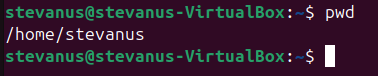
\includegraphics[width=0.75\textwidth]{Figure/03/gambar1.png}
            \caption{Tampilan terminal saat memverifikasi lokasi direktori menggunakan perintah \texttt{pwd}.}
            \label{fig:m03-gambar1}
        \end{figure}
    \end{enumerate}

    \vspace{1em}
    \item \textbf{Manipulasi Direktori dan Berkas}
    
    Pada tahap ini, Anda akan membuat, menyalin, dan memindahkan berkas menggunakan perintah dasar CLI.
    \begin{enumerate}
        \item Buatlah sebuah direktori baru bernama \texttt{data} dan masuk ke dalamnya menggunakan perintah \texttt{cd}.
        \begin{lstlisting}[language=bash, caption={Membuat dan masuk ke direktori baru}]
    $ mkdir data
    $ cd data
        \end{lstlisting}
        \begin{figure}[H]
            \centering
            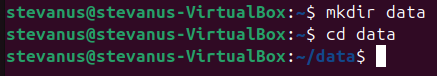
\includegraphics[width=0.75\textwidth]{Figure/03/gambar2.png}
            \caption{Proses pembuatan direktori baru dan berpindah ke dalamnya.}
            \label{fig:m03-gambar2}
        \end{figure}
        
        \item Buatlah berkas teks baru menggunakan teks editor \texttt{nano}.
        \begin{lstlisting}[language=bash, caption={Membuka editor nano}]
    $ nano belajarlinux.txt
        \end{lstlisting}
        Ketikkan Nama dan NIM Anda di dalamnya. Simpan perubahan dengan menekan \texttt{Ctrl+O} lalu tekan \texttt{Enter}. Setelah itu, keluar dari editor dengan menekan \texttt{Ctrl+X}.
        \begin{figure}[H]
            \centering
            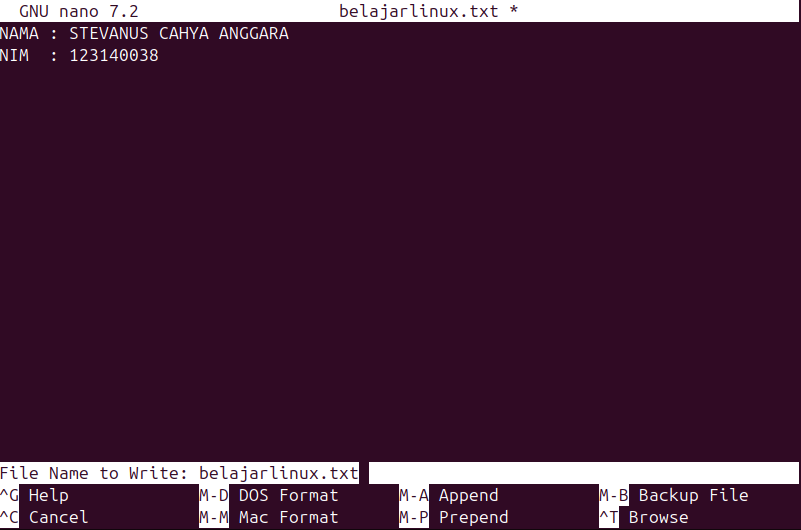
\includegraphics[width=0.75\textwidth]{Figure/03/gambar4.png}
            \caption{Tampilan editor teks \texttt{nano} saat mengedit berkas.}
            \label{fig:m03-gambar3}
        \end{figure}
        
        \item Tampilkan isi berkas yang baru saja dibuat ke layar terminal menggunakan perintah \texttt{cat}.
        \begin{lstlisting}[language=bash, caption={Menampilkan isi berkas}]
    $ cat belajarlinux.txt
        \end{lstlisting}
        Isi berkas akan langsung tercetak di terminal. Contoh output sesuai data yang Anda masukkan:
        \begin{lstlisting}[language=bash]
    Nama: Budi Santoso
    NIM: 12345678
        \end{lstlisting}

        \item Buat direktori baru bernama \texttt{data2} dan salin berkas \texttt{belajarlinux.txt} ke dalamnya.
        \begin{lstlisting}[language=bash, caption={Menyalin berkas menggunakan cp}]
    $ mkdir data2
    $ cp belajarlinux.txt data2/
    $ ls data2/
        \end{lstlisting}
        \begin{figure}[H]
            \centering
            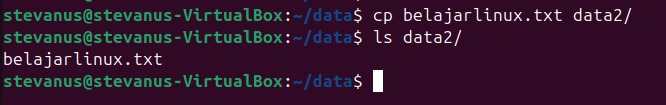
\includegraphics[width=0.75\textwidth]{Figure/03/gambar5.png}
            \caption{Proses penyalinan berkas ke dalam direktori tujuan beserta verifikasinya.}
            \label{fig:m03-gambar5}
        \end{figure}
        
        \item Pindah ke direktori \texttt{data2} dan ubah nama berkas menggunakan perintah \texttt{mv}.
        \begin{lstlisting}[language=bash, caption={Mengubah nama berkas menggunakan mv}]
    $ cd data2
    $ mv belajarlinux.txt belajarlagi.txt
    $ ls
        \end{lstlisting}
        \begin{figure}[H]
            \centering
            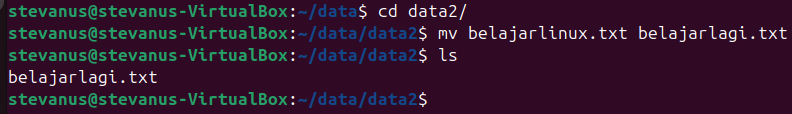
\includegraphics[width=0.75\textwidth]{Figure/03/gambar6.png}
            \caption{Pengubahan nama berkas menggunakan perintah \texttt{mv}.}
            \label{fig:m03-gambar6}
        \end{figure}
    \end{enumerate}

    \vspace{1em}
    \item \textbf{Manipulasi Hak Akses}
    
    Pada tahap ini, Anda akan mencoba mengubah "kunci gembok" (\textit{permissions}) dari berkas yang sudah dibuat sebelumnya. 
    \begin{enumerate}
        \item Hapus hak akses baca (\textit{read}) dan tulis (\textit{write}) untuk pengguna asing (\textit{others}) pada berkas \texttt{belajarlagi.txt} dengan menggunakan parameter \texttt{o-rw}.
        \begin{lstlisting}[language=bash, caption={Mengubah hak akses berkas (symbolic mode)}]
    $ chmod o-rw belajarlagi.txt

    # Verifikasi perubahan hak akses, perhatikan deretan huruf di sebelah kiri
    $ ls -l
        \end{lstlisting}

        \noindent\textbf{Catatan — Mode Numerik (Oktal):} Perintah di atas menggunakan \textit{symbolic mode}. Perintah yang sama dapat ditulis dengan \textit{numeric mode} menggunakan angka oktal dari tabel \ref{tab:chmod-oktal}. Sebagai contoh, \texttt{chmod 640 belajarlagi.txt} memberikan efek yang setara:
        \begin{itemize}
            \item \textbf{6} (4+2) $\rightarrow$ \textit{Owner}: baca dan tulis (\texttt{rw-})
            \item \textbf{4} $\rightarrow$ \textit{Group}: hanya baca (\texttt{r--})
            \item \textbf{0} $\rightarrow$ \textit{Others}: tanpa akses (\texttt{---})
        \end{itemize}
        \begin{lstlisting}[language=bash, caption={Perintah yang setara menggunakan numeric mode}]
    $ chmod 640 belajarlagi.txt
        \end{lstlisting}
        \begin{figure}[H]
            \centering
            
\includegraphics[width=0.75\textwidth]{Figure/03/gambar7.png}
            \caption{Status hak akses berkas sebelum dilakukan modifikasi.}
            \label{fig:m03-gambar7}
        \end{figure}
        \begin{figure}[H]
            \centering
            
\includegraphics[width=0.75\textwidth]{Figure/03/gambar8.png}
            \caption{Status hak akses berkas setelah modifikasi dengan \texttt{chmod}.}
            \label{fig:m03-gambar8}
        \end{figure}
        
        \item Coba ubah kepemilikan berkas tersebut menjadi milik pengguna \texttt{root}.

        Operasi \texttt{chown} (change owner) mengubah siapa yang tercatat sebagai \textit{owner} dari sebuah berkas. Karena mengubah kepemilikan merupakan tindakan administratif yang berdampak pada keamanan sistem, perintah ini \textbf{memerlukan hak} \textit{superuser} dan harus dijalankan dengan \texttt{sudo}.
        \begin{lstlisting}[language=bash, caption={Menggunakan sudo untuk mengubah owner ke root}]
    $ sudo chown root belajarlagi.txt
    $ ls -l
        \end{lstlisting}
        Setelah perintah ini, kolom kepemilikan pada output \texttt{ls -l} akan berubah dari nama pengguna Anda menjadi \texttt{root}. Akibatnya, Anda \textbf{tidak lagi dapat mengedit} berkas tersebut tanpa menggunakan \texttt{sudo}, karena \textit{owner}-nya kini bukan Anda.

        Untuk mengembalikan kepemilikan ke pengguna Anda sendiri, jalankan:
        \begin{lstlisting}[language=bash, caption={Mengembalikan kepemilikan berkas ke pengguna semula}]
    $ sudo chown $USER belajarlagi.txt
        \end{lstlisting}
        Variabel \texttt{\$USER} secara otomatis merujuk ke nama pengguna yang sedang aktif.
        \begin{figure}[H]
            \centering
            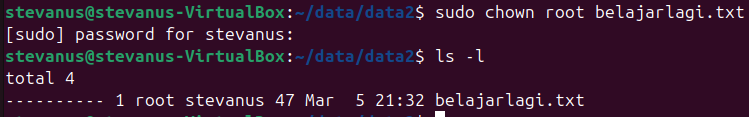
\includegraphics[width=0.75\textwidth]{Figure/03/gambar9.png}
            \caption{Perubahan kepemilikan berkas menjadi pengguna \texttt{root}.}
            \label{fig:m03-gambar9}
        \end{figure}
    \end{enumerate}

\end{enumerate}

% --- 5. Penanganan Kesalahan Umum ---
\newpage
\section{Penanganan Kesalahan Umum}
\label{sec:m03-troubleshooting}

Berikut adalah pesan kesalahan yang sering dijumpai selama praktikum beserta cara mengatasinya:

\begin{table}[H]
    \caption{Kesalahan Umum dan Cara Mengatasinya}
    \label{tab:m03-troubleshooting}
    \centering
    \begin{tabular}{|p{5.5cm}|p{4cm}|p{4.5cm}|}
        \hline
        \textbf{Pesan Kesalahan} & \textbf{Penyebab Umum} & \textbf{Cara Mengatasi} \\ \hline
        \texttt{Permission denied} & Anda tidak memiliki hak akses untuk membaca, menulis, atau menjalankan berkas tersebut. & Periksa permission dengan \texttt{ls -l}. Gunakan \texttt{chmod} untuk menyesuaikan, atau tambahkan \texttt{sudo} jika aksi memerlukan hak administratif. \\ \hline
        \texttt{mkdir: cannot create directory 'data': File exists} & Direktori dengan nama yang sama sudah ada. & Gunakan nama direktori lain, atau hapus direktori lama terlebih dahulu dengan \texttt{rm -r namadir}. \\ \hline
        \texttt{No such file or directory} & Berkas atau direktori yang dituju tidak ditemukan di \textit{path} yang diberikan. & Pastikan ejaan nama berkas benar. Gunakan \texttt{ls} untuk melihat isi direktori saat ini, dan \texttt{pwd} untuk mengecek lokasi Anda. \\ \hline
        \texttt{sudo: command not found} & Perintah \texttt{sudo} tidak tersedia (jarang terjadi di Ubuntu). & Pastikan Anda menggunakan distribusi Ubuntu yang sudah dikonfigurasi. Hubungi asisten praktikum jika masalah berlanjut. \\ \hline
        \texttt{bash: nano: command not found} & Editor \texttt{nano} belum terpasang. & Pasang dengan perintah \texttt{sudo apt install nano}. \\ \hline
    \end{tabular}
\end{table}
% ============================================================
%  Modul 4 — Automasi dengan Bash Scripting
% ============================================================

\chapter{Automasi Bash Scripting}
\label{chap:modul-04}

% --- 1. Tujuan dan Output Praktikum ---
\section{Tujuan dan Output Praktikum}

\subsection{Tujuan Praktikum}
Setelah menyelesaikan praktikum ini, mahasiswa diharapkan mampu:
\begin{enumerate}
	\item Menjelaskan konsep dasar \textit{shell scripting} dan perannya dalam proses automasi sistem operasi.
	\item Memahami sintaks dasar skrip \textit{bash}, termasuk pemanfaatan variabel dan deklarasi \textit{shebang}.
	\item Membuat \textit{Shell Script} (.sh) sederhana dengan menggabungkan perintah-perintah dasar sistem file Linux seperti \texttt{mkdir}, \texttt{cp}, dan \texttt{cat} \cite{shotts2019linux}.
	\item Memberikan dan mengeksekusi hak akses (\textit{execute permissions}) pada skrip agar dapat dijalankan secara legal oleh sistem operasi.
\end{enumerate}

\subsection{Output Praktikum}
Pada akhir praktikum ini, mahasiswa diharapkan menghasilkan:
\begin{itemize}
	\item File \textit{shell script} berekstensi \texttt{.sh} yang memuat rangkaian instruksi automasi \textit{backup}.
	\item Direktori cadangan (\textit{backup}) yang tercipta secara otomatis dari hasil eksekusi skrip tersebut.
	\item Dokumentasi verifikasi keberhasilan pemberian izin status \textit{executable} pada file skrip.
\end{itemize}

% --- 2. Dasar Teori ---
\newpage
\section{Dasar Teori}

\subsection{Pengantar Automasi dan Bash Scripting}
\textit{Shell Scripting} adalah proses penggabungan serangkaian instruksi baris perintah (CLI) ke dalam sebuah teks file murni yang nantinya akan dieksekusi secara otomatis oleh penerjemah sistem (\textit{shell}). Pada Linux, setiap perintah dieksekusi melalui shell, yaitu program yang menyediakan lingkungan kerja bagi pengguna untuk berinteraksi dengan sistem operasi \cite{robbins2005classic}. 

Secara analogi, bayangkan sistem operasi Linux Anda sebagai seorang koki. Mengetik perintah satu per satu di terminal ibarat Anda berdiri di dapur dan mendiktekan instruksi memasak kalimat demi kalimat. Hal ini efisien untuk masakan sederhana, namun melelahkan untuk tugas rumit. Sebaliknya, \textit{Shell Scripting} ibarat Anda menyusun "Resep Masakan" utuh di secarik kertas, di mana instruksi seperti menyalin file (\texttt{cp}) atau memindahkan direktori (\texttt{mv}) dapat dijalankan secara mandiri dan konsisten dari awal hingga selesai \cite{das2012unix}.

\subsection{Struktur Skrip: Shebang dan Variabel}
Sebuah \textit{shell script} yang terstandarisasi selalu diawali dengan rangkaian karakter khusus yang disebut \textbf{Shebang} (\texttt{\#!/bin/bash}). Baris pertama ini adalah pengarah yang memberitahu \textit{kernel} sistem operasi tentang program mana yang harus dipanggil untuk memproses baris-baris instruksi di bawahnya.

Untuk menyimpan data yang dinamis di dalam skrip, kita menggunakan \textbf{variabel}. Variabel bertindak sebagai "kotak wadah berlabel". Alih-alih mengingat dan mengetikkan teks \textit{path} direktori yang panjang berkali-kali, kita cukup menyimpan teks tersebut ke dalam sebuah variabel dan hanya memanggil namanya saja saat kode dieksekusi.

\subsection{Automasi Backup dan Hak Eksekusi (Execute)}
Tugas administrasi yang paling sering dijadikan kandidat automasi adalah pencadangan (\textit{backup}) direktori. Namun, file skrip teks biasa tidak akan pernah bisa dijalankan sebagai program langsung oleh Linux demi meminimalisasi insiden keamanan. 

Kita harus secara eksplisit menambahkan hak akses eksekusi (\textit{execute permissions}) menggunakan sintaks flag modifikasi pada perintah \texttt{chmod}. Jika eksekusi gagal, sering kali kita harus memastikan kembali apakah kita mengeksekusi skrip tersebut pada tingkatan \textit{user} biasa (\texttt{\$}) atau membutuhkan privilese \textit{root} (\texttt{\#}) menggunakan \texttt{sudo} \cite{shotts2019linux}.

\begin{table}[H]
	\caption{Tabel Ringkasan Operasi Shell Scripting}
	\label{tab:m04-dasar-teori}
	\centering
	\begin{tabular}{|l|p{9cm}|}
		\hline
		\textbf{Sintaks} & \textbf{Penjelasan Singkat} \\ \hline
		\texttt{\#!/bin/bash} & \textit{Shebang}, wajib berada di baris pertama skrip. \\ \hline
		\texttt{NAMA="Data"} & Deklarasi variabel tanpa spasi. \\ \hline
		\texttt{echo} & Menampilkan string atau isi variabel ke layar terminal. \\ \hline
		\texttt{cp -r} & Menyalin direktori beserta seluruh isinya secara rekursif. \\ \hline
		\texttt{chmod +x} & Menambahkan hak eksekusi file. \\ \hline
		\texttt{./skrip.sh} & Menjalankan eksekusi skrip di lokasi \textit{Current Directory} saat ini. \\ \hline
	\end{tabular}
\end{table}

% --- 3. Alat dan Bahan ---
\newpage
\section{Alat dan Bahan}
\label{sec:m04-alat-bahan}

\subsection{Perangkat Keras}
\begin{itemize}
	\item Laptop atau PC dengan prosesor minimal \textit{dual-core}.
	\item RAM minimal 4 GB.
\end{itemize}

\subsection{Perangkat Lunak}
\begin{itemize}
	\item Oracle VM VirtualBox dengan OS tamu Linux.
	\item Teks Editor baris perintah \texttt{nano}.
\end{itemize}

% --- 4. Langkah-Langkah Praktikum ---
\newpage
\section{Langkah-Langkah Praktikum}

\subsection{Persiapan Data Target}
\label{sec:m04-persiapan}
Untuk mensimulasikan proses \textit{backup}, kita perlu membuat struktur data uji menggunakan perintah membuat direktori baru (\texttt{mkdir}).

\begin{enumerate}
	\item Buka terminal Linux dengan \texttt{Ctrl+Alt+T}, kemudian siapkan direktori target.
	\begin{lstlisting}[language=bash, caption={Menyiapkan direktori uji}]
		$ mkdir Data_Penting
		$ echo "Simulasi data keuangan." > Data_Penting/keuangan.txt
		$ echo "Simulasi daftar mahasiswa." > Data_Penting/mahasiswa.txt
	\end{lstlisting}
\end{enumerate}

\begin{figure}[H]
	\centering
	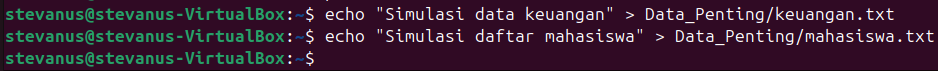
\includegraphics[width=0.75\textwidth]{Figure/04/gambar10.png}
	\caption{Proses penyiapan direktori dan data simulasi untuk target \textit{backup}.}
	\label{fig:m04-gambar10}
\end{figure}

\subsection{Sesi 1: Penulisan Skrip Bash Sederhana}
\label{sec:m04-sesi-1}

\begin{enumerate}
	\item Gunakan editor teks \texttt{nano} untuk membuat file berakhiran \texttt{.sh}.
	\begin{lstlisting}[language=bash, caption={Membuka editor nano}]
		$ nano script_backup.sh
	\end{lstlisting}
	
	\item Di dalam \textit{workspace nano}, ketikkan baris skrip di bawah ini. Jika sudah, simpan dengan menekan \texttt{Ctrl+O}, \texttt{Enter}, lalu \texttt{Ctrl+X} untuk menutup.
	\begin{lstlisting}[language=bash, caption={Struktur Skrip Automasi Backup Sederhana}]
		#!/bin/bash
		# Automasi proses duplikasi keamanan data
		
		SUMBER="Data_Penting"
		TUJUAN="Backup_$(date +%F)"
		
		echo "Sedang menyalin direktori: $SUMBER..."
		
		# Eksekusi proses copy rekursif ke variabel TUJUAN
		cp -r $SUMBER $TUJUAN
		
		echo "Proses backup selesai! Tersimpan di: $TUJUAN"
	\end{lstlisting}
\end{enumerate}

\begin{figure}[H]
	\centering
	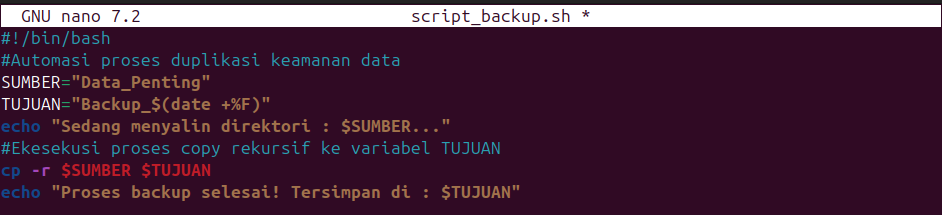
\includegraphics[width=0.75\textwidth]{Figure/04/gambar11.png}
	\caption{Tampilan penulisan skrip \textit{backup} memanfaatkan teks editor CLI terintegrasi.}
	\label{fig:m04-gambar11}
\end{figure}

\subsection{Sesi 2: Manipulasi Izin Execute dan Menjalankan Skrip}
\label{sec:m04-sesi-2}

\begin{enumerate}
	\item Berikan izin \textit{executable} pada file skrip. 
	\begin{lstlisting}[language=bash, caption={Memberikan izin eksekusi ke file script}]
		# Mengecek metadata dan izin file awal sebelum dimodifikasi
		$ ls -l script_backup.sh
		
		# Menambahkan modifier executable (+x)
		$ chmod +x script_backup.sh
		
		# Mengecek kembali, file akan berubah warna
		$ ls -l script_backup.sh
	\end{lstlisting}
	
	\item Panggil nama skrip tersebut dan verifikasi eksekusinya.
	\begin{lstlisting}[language=bash, caption={Eksekusi program bash}]
		# Menjalankan script di folder saat ini (./)
		$ ./script_backup.sh
		
		# Memeriksa hasil backup menggunakan perintah ls
		$ ls -l
	\end{lstlisting}
\end{enumerate}

\begin{figure}[H]
	\centering
	
\includegraphics[width=0.75\textwidth]{Figure/04/gambar12.png}
	\caption{Validasi proses modifikasi izin eksekusi dan keberhasilan eksekusi automasi \textit{backup} pada terminal.}
	\label{fig:m04-gambar12}
\end{figure}

\newpage
\section{\textit{Hands On}}
\label{sec:m04-hands-on}

Pada bagian ini, setiap mahasiswa wajib mengerjakan tugas praktik mandiri yang mencakup materi pemahaman dari Modul 3 dan Modul 4 sebagai berikut:

\begin{enumerate}
	\item Buatlah struktur direktori berikut secara berurutan:
	\begin{itemize}
		\item Buat 2 direktori bernama \texttt{mahasiswa\_namaanda} dan \texttt{matakuliah\_namaanda}.
		\item Di dalam \texttt{mahasiswa\_namaanda}, buat file teks menggunakan \texttt{nano} bernama \texttt{datadiri\_namaanda.txt} yang berisi Nama, NIM, Prodi, dan Angkatan Anda.
		\item Di dalam \texttt{matakuliah\_namaanda}, buat file teks bernama \texttt{sistemoperasi\_namaanda.txt} yang memuat Nama, Kelas, dan Kode IF.
	\end{itemize}
	\item Pindahkan seluruh folder \texttt{matakuliah\_namaanda} ke dalam folder \texttt{mahasiswa\_namaanda} menggunakan perintah \texttt{mv}. Tampilkan isi file \texttt{sistemoperasi\_namaanda.txt} di terminal menggunakan \texttt{cat}.
	\item Demonstrasikan modifikasi hak akses dengan menghapus izin \textit{write} (\texttt{w}) pada file \texttt{datadiri\_namaanda.txt} menggunakan \texttt{chmod}.
	\item Susun sebuah \textit{shell script} (\texttt{backup\_tugas.sh}) yang akan mengotomatisasi penyalinan (\texttt{cp}) folder \texttt{mahasiswa\_namaanda} ke sebuah folder baru bernama \texttt{Arsip\_namaanda}.
	\item Berikan izin eksekusi (\texttt{chmod +x}) pada skrip tersebut dan jalankan skripnya di terminal. Verifikasi apakah folder arsip terbentuk dengan benar.
	\item Dokumentasikan setiap langkah dan perintah eksekusi terminal secara berurutan (wajib disertai \textit{screenshot}).
	\item Menyusun laporan praktikum sesuai \textit{template} resmi pada GitHub IF ITERA: \\
	\url{https://github.com/informatika-itera/IF25-12007-Sistem-Operasi/tree/main/Hands-On}
\end{enumerate}

Laporan \textbf{wajib} disusun menggunakan \LaTeX.
% % ============================================================
%  Modul 5 — Sistem Build dengan GCC
% ============================================================

\chapter{Sistem Build dengan GCC}
\label{chap:modul-05}

% --- 1. Tujuan dan Output Praktikum ---
\section{Tujuan dan Output Praktikum}

\subsection{Tujuan Praktikum}
Setelah menyelesaikan praktikum ini, mahasiswa diharapkan mampu:
\begin{enumerate}
	\item Memahami proses kompilasi kode sumber C/C++ menggunakan \textit{GNU Compiler Collection} (GCC).
	\item Mengenal dan mempraktikkan tahapan dalam proses \textit{build}: preparasi, kompilasi, perakitan (\textit{assembly}), dan \textit{linking}.
\end{enumerate}

\subsection{Output Praktikum}
Pada akhir praktikum ini, mahasiswa diharapkan menghasilkan:
\begin{itemize}
	\item File kode sumber C sederhana yang berhasil dikompilasi menjadi \textit{executable}.
	\item Hasil dari setiap tahapan proses kompilasi (\texttt{.i}, \texttt{.s}, \texttt{.o}).
\end{itemize}

% --- 2. Dasar Teori ---
\newpage
\section{Dasar Teori}

\subsection{GNU Compiler Collection (GCC)}
GCC awalnya merupakan \textit{GNU C Compiler}, namun kini telah berkembang mendukung berbagai bahasa pemrograman seperti C, C++, Objective-C, Fortran, Ada, Go, dan D \cite{gough2004introduction}. GCC adalah standar kompiler yang banyak digunakan dalam sistem operasi mirip UNIX (Unix-like), terutama distribusi Linux. GCC dirancang agar kuat, fleksibel, teroptimasi, dan mendukung banyak arsitektur perangkat keras.

\subsection{Tahapan Kompilasi GCC}
Proses mengubah (\textit{build}) suatu kode sumber bahasa tingkat tinggi (seperti C) menjadi program (\textit{executable}) yang bisa dijalankan komputer dilakukan melalui 4 proses sekuensial \cite{bryant2015computer}:

\subsubsection{Preprocessing (Pra-kompilasi)}
Pada tahap ini, kompiler menginisialisasi pengerjaan arahan preprosesor (seperti \texttt{\#include}, \texttt{\#define}). Ia menambahkan kode dari \textit{header file}, mengganti makro, dan membuang komentar pada kode sumber awal (misal \texttt{main.c}). Tahapan ini mendayagunakan perangkat lunak \textit{C Preprocessor} (\texttt{cpp}) dan menghasilkan file berekstensi \texttt{.i}.

\subsubsection{Compilation (Kompilasi)}
Tahap ini mengambil keluaran dari preprosesor (\texttt{.i}) lalu menerjemahkannya ke dalam kode bahasa rakitan (\textit{assembly language}) spesifik sesuai arsitektur mesin tujuan. Hasil dari tahap kompilasi ini adalah sebuah teks instruksi assembli berekstensi \texttt{.s}.

\subsubsection{Assembly (Perakitan)}
Kode \textit{assembly} (\texttt{.s}) diproses ke dalam bahasa mesin (\textit{machine level language} berformat biner) yang dapat dimengerti sistem komputer. Perangkat lunak yang merangkap proses ini disebut \textit{Assembler} (\texttt{as}). Output dari tahapan ini adalah file objek (\textit{object file}) berekstensi \texttt{.o}. File ini masih belum bisa dieksekusi sebelum dihubungkan dengan library atau file objek lain.

\subsubsection{Linking (Penautan)}
Fase terakhir merupakan tahap penggabungan di mana berbagai file objek pendukung (\texttt{.o}) disatukan menjadi satu program utuh beserta file pustaka bawaan (\textit{library file}). Contoh umum adalah penautan dengan glibc (standar pustaka C). Jika menggunakan pustaka pihak ketiga semisal \textit{math} atau \textit{pthread}, tautannya juga dideklarasikan di sini (\texttt{-lm}, \texttt{-lpthread}). Perangkat lunaknya dinamai \textit{Linker} (\texttt{ld}). Outputnya adalah file \textit{executable}.

Tabel \ref{tab:m05-dasar-teori} merangkum hal-hal penting terkait flag GCC yang sering digunakan.

\begin{table}[h]
	\caption{Ringkasan Flag GCC Umum}
	\label{tab:m05-dasar-teori}
	\centering
	\begin{tabulary}{\textwidth}{|L|L|}
		\hline
		\textbf{Flag} & \textbf{Penjelasan Singkat} \\ \hline
		\texttt{-o}     & Spesifikasikan nama file output \\ \hline
		\texttt{-Wall}  & Nyalakan peringatan kompilator ("Wall" = Warning all) \\ \hline
		\texttt{-E}     & Berhenti setelah tahap Preprocessing tanpa melakukan yang lain \\ \hline
		\texttt{-S}     & Hasilkan file .s, jangan assemble (berhenti di tahap Compilation) \\ \hline
		\texttt{-c}     & Menghasilkan file output berbentuk assembli murni atau .o (berhenti di tahap Assembly) \\ \hline
		\texttt{-g}     & Sertakan informasi \textit{debugging} (berguna menggunakan GDB) \\ \hline
	\end{tabulary}
\end{table}

% --- 3. Alat dan Bahan ---
\newpage
\section{Alat dan Bahan}
\label{sec:m05-alat-bahan}

\subsection{Perangkat Keras}
\begin{itemize}
	\item PC/Laptop dengan arsitektur prosesor x86\_64 atau lainnya.
	\item Ruang penyimpanan yang cukup untuk menyimpan hasil \textit{build}.
\end{itemize}

\subsection{Perangkat Lunak}
\begin{itemize}
	\item Sistem Operasi berbasis Linux (Ubuntu Desktop/Server) atau WSL 2.
	\item Instalasi \textit{build-essential} (mencakup \texttt{gcc}, \texttt{make}, dan lainnya).
	\item Kode editor (seperti Vim, Nano, atau VS Code).
\end{itemize}

% --- 4. Langkah-Langkah Praktikum ---
\newpage
\section{Langkah-Langkah Praktikum}

\subsection{Persiapan Lingkungan}
\label{sec:m05-persiapan}
Sebelum memulai kompilasi, pastikan lingkungan memadai dan gcc sudah diatur dengan benar di dalam sistem Anda.

Berikut adalah tahapan-tahapan yang harus Anda selesaikan secara berurutan:

\begin{enumerate}
	\item Buka terminal (atau distro WSL yang telah Anda konfigurasikan).
	\item Pastikan instrumen penunjang sudah ter-install dengan paket yang disarankan (\textit{build-essential}).
	      \begin{lstlisting}[language=bash, caption={Perintah verifikasi lingkungan}]
sudo apt update
sudo apt install build-essential -y
gcc --version
make --version
    \end{lstlisting}

	      \begin{figure}[htbp]
		      \centering
		      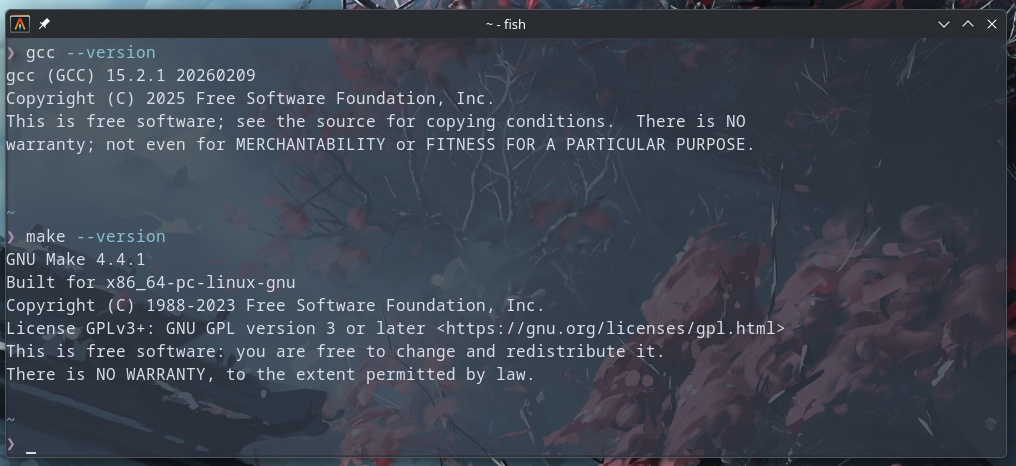
\includegraphics[width=0.75\textwidth]{Figure/05/gcc-make.png}
		      \caption{Verifikasi Versi GCC dan Make}
		      \label{fig:m05-gcc-make}
	      \end{figure}

	\item Buat sebuah direktori bernama \texttt{praktikum-gcc} untuk praktikum modul ini.
	      \begin{lstlisting}[language=bash, caption={Membuat direktori kerja}]
mkdir praktikum-gcc
cd praktikum-gcc
    \end{lstlisting}
\end{enumerate}

\subsection{Sesi 1: Siklus Hidup Kompilasi C}
\label{sec:m05-sesi-1}
Kita akan membongkar proses kompilasi penuh sebuah program C sederhana menggunakan sekumpulan \textit{flags} untuk menangguhkan setiap tahapan \textit{build}, sehingga Anda dapat memahaminya secara parsial.

Berikut adalah tahapan-tahapan yang harus Anda selesaikan secara berurutan:

\begin{enumerate}
	\item Buatlah sebuah file kode sumber C bernama \texttt{salam.c} menggunakan teks editor terminal \texttt{nano}:
	      \begin{lstlisting}[language=bash, caption={Membuat file dengan nano}]
nano salam.c
    \end{lstlisting}

	\item Di dalam \texttt{nano}, ketik atau salin kode bahasa C berikut:
	      \begin{lstlisting}[language=c, caption={Isi salam.c}]
#include <stdio.h>
#define PESAN "Halo, Selamat datang di Pembelajaran Sistem Operasi!"

int main() {
    printf("%s\n", PESAN);
    return 0;
}
    \end{lstlisting}
	      \textit{Simpan file di nano dengan menekan Ctrl+O, lalu Enter. Kemudian keluar dengan Ctrl+X.}

	      \begin{figure}[H]
		      \centering
		      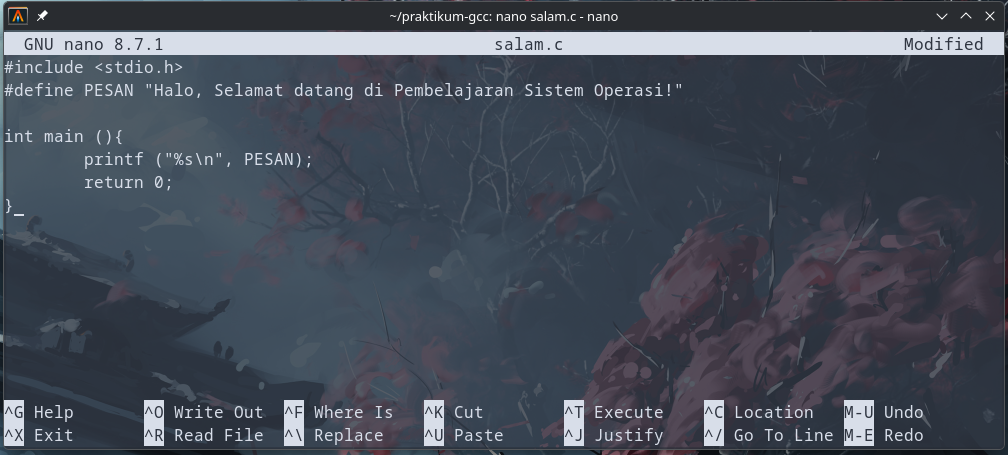
\includegraphics[width=0.75\textwidth]{Figure/05/nano-salam-c.png}
		      \caption{Membuat file salam.c dengan Nano}
		      \label{fig:m05-nano-salam-c}
	      \end{figure}

	\item Praktikkan tahapan pertama, yaitu \textbf{Preprocessing} (menginisialisasi header dan macro) secara manual dengan argumen (\texttt{-E}):
	      \begin{lstlisting}[language=bash, caption={Preprocessing}]
gcc -E salam.c -o salam.i
    \end{lstlisting}
	      Anda bisa melihat isi dari file hasil prakompilasi dengan \texttt{cat salam.i} atau \texttt{less salam.i}. Gulir ke bawah (atau tekan spasi di `less`), akan tampak baris macro `PESAN` telah diubah dengan nilai aslinya.

	      \begin{figure}[H]
		      \centering
		      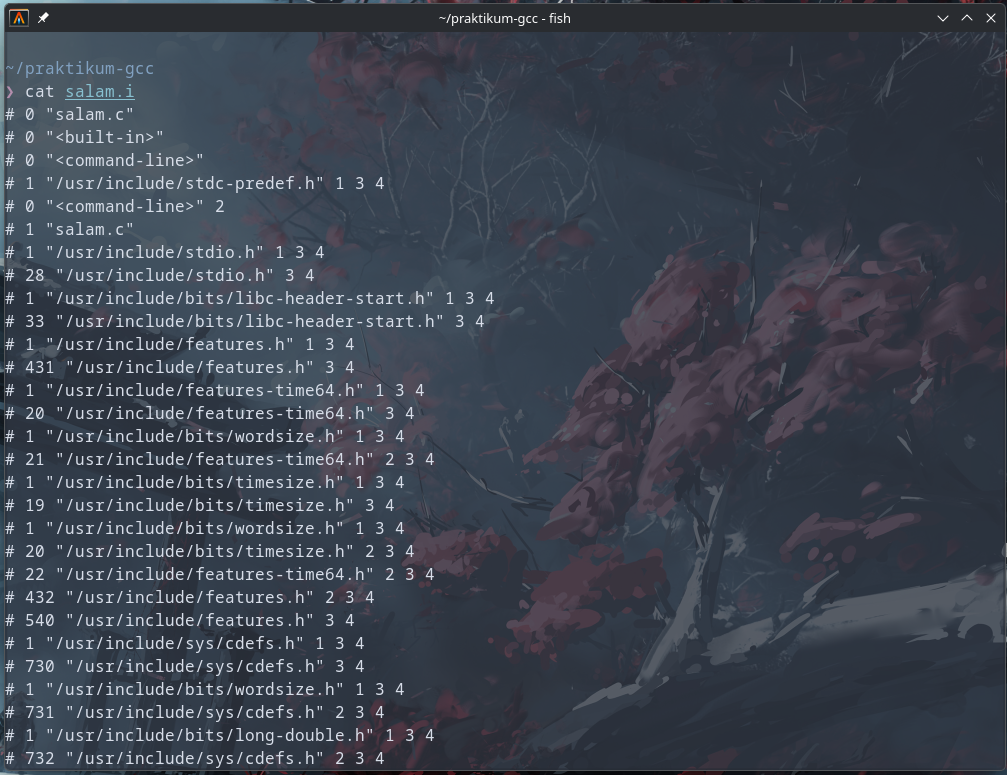
\includegraphics[width=0.75\textwidth]{Figure/05/salam-i.png}
		      \caption{Hasil Preprocessing}
		      \label{fig:m05-salam-i}
	      \end{figure}

	\item Praktikkan tahapan \textbf{Compilation} yang mengubahnya menjadi bahasa mesin/assembly (\texttt{-S}):
	      \begin{lstlisting}[language=bash, caption={Kompilasi menjadi Assembly}]
gcc -S salam.c -o salam.s
cat salam.s
    \end{lstlisting}
	      Teks output `cat` akan memunculkan instruksi-instruksi CPU yang rumit. Inilah yang disebut \textbf{assembly}.

	      \begin{figure}[H]
		      \centering
		      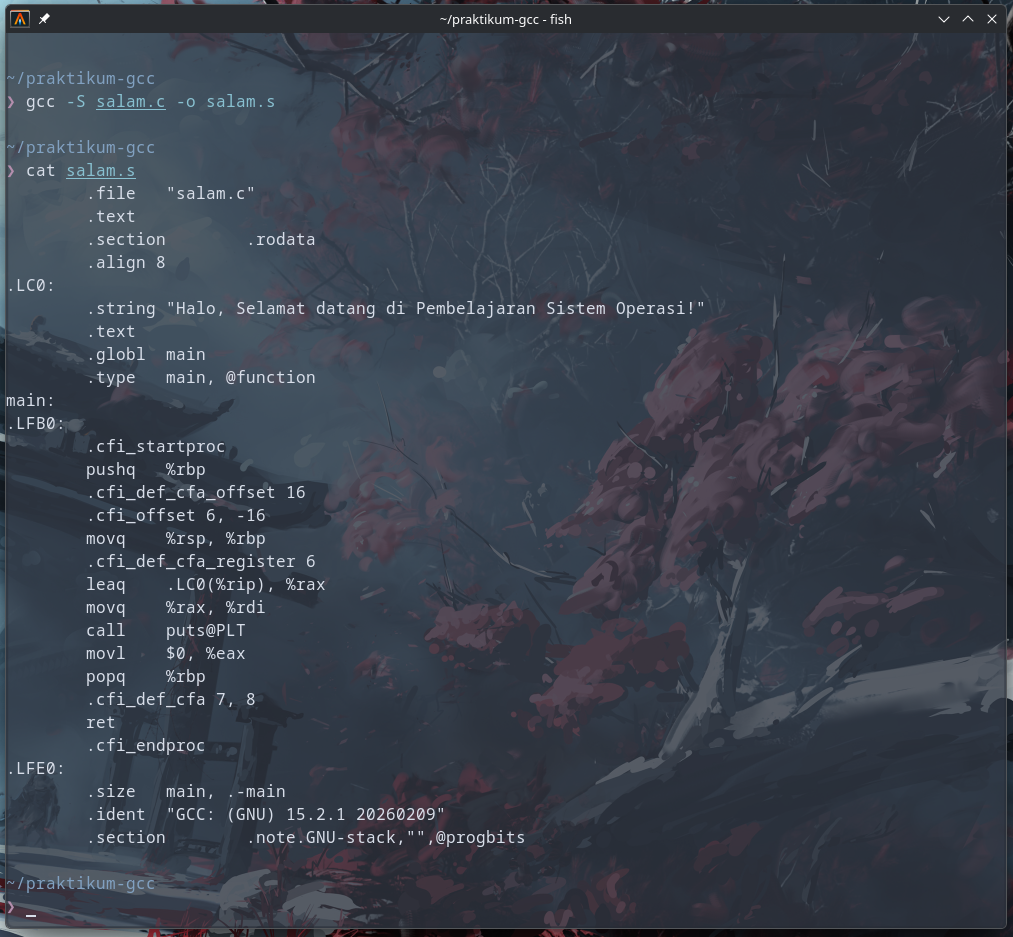
\includegraphics[width=0.75\textwidth]{Figure/05/salam-s.png}
		      \caption{Hasil Compilation}
		      \label{fig:m05-salam-s}
	      \end{figure}

	\item Praktikkan tahapan \textbf{Assembly} untuk merakitnya menjadi \textit{object file} biner (\texttt{-c}):
	      \begin{lstlisting}[language=bash, caption={Assemble menjadi file objek}]
gcc -c salam.c -o salam.o
    \end{lstlisting}
	      \textit{object file}  (\texttt{.o}) ini bukan lagi sebuah teks ASCII yang bisa dibaca manusia, ini adalah sebuah format instruksi mesin dalam bentuk biner. Anda tidak perlu membacanya dengan `cat`.

	      \begin{figure}[H]
		      \centering
		      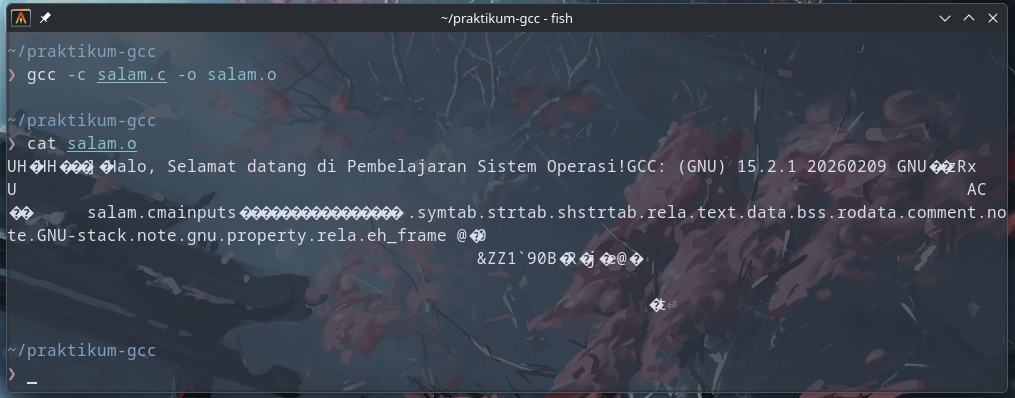
\includegraphics[width=0.75\textwidth]{Figure/05/salam-o.png}
		      \caption{Hasil Assembly}
		      \label{fig:m05-salam-o}
	      \end{figure}

	\item Tahap akhir, praktikkan \textbf{Linking} sebagai jembatan yang menyatukan semua kode objek dengan file pustaka internal menjadi file yang siap jalan (\texttt{Executable}):
	      \begin{lstlisting}[language=bash, caption={Linking menjadi Executable}]
gcc salam.o -o program_salam
    \end{lstlisting}

	\item Sekarang Anda bisa langsung mencoba menjalankan (run) file executablenya:
	      \begin{lstlisting}[language=bash, caption={Eksekusi program}]
./program_salam
    \end{lstlisting}
	      Hasilnya akan menampilkan pesan `Halo, Selamat datang di Pembelajaran Sistem Operasi!` di terminal.

	      \begin{figure}[H]
		      \centering
		      
\includegraphics[width=0.75\textwidth]{Figure/05/program-salam.png}
		      \caption{Hasil Eksekusi Program Salam}
		      \label{fig:m05-program-salam}
	      \end{figure}
\end{enumerate}
% % ============================================================
%  Modul 6 — Otomatisasi Proses Build dengan Makefile
% ============================================================

\chapter{Otomatisasi Proses Build dengan Makefile}
\label{chap:modul-06}

% --- 1. Tujuan dan Output Praktikum ---
\section{Tujuan dan Output Praktikum}

\subsection{Tujuan Praktikum}
Setelah menyelesaikan praktikum ini, mahasiswa diharapkan mampu:
\begin{enumerate}
    \item Memahami konsep dasar otomatisasi kompilasi (\textit{build automation}) perangkat lunak.
    \item Memahami dan menjelaskan struktur dasar berkas \texttt{Makefile} (Target, Komponen Syarat, dan Resep).
    \item Menggunakan variabel kompilator dan \textit{flags} penanda dalam \texttt{Makefile}.
    \item Menggunakan variabel otomatis (\textit{automatic variables}) seperti \texttt{\$@} dan \texttt{\$\textasciicircum} untuk efisiensi skrip \textit{build}.
\end{enumerate}

\subsection{Output Praktikum}
Pada akhir praktikum ini, mahasiswa diharapkan menghasilkan:
\begin{itemize}
    \item Berkas \texttt{Makefile} yang mampu mengompilasi program dengan satu ketikan perintah.
    \item Berkas \texttt{Makefile} multi-target (termasuk fitur \texttt{clean} untuk membersihkan proyek).
    \item Kode program multi-berkas yang sukses dikompilasi menggunakan aturan \texttt{Makefile} tingkat lanjut.
\end{itemize}

% --- 2. Dasar Teori ---
\newpage
\section{Dasar Teori}

\subsection{Otomatisasi Build dan Utilitas Make}
Dalam pengembangan perangkat lunak modern, sebuah program sering kali bersumber dari ratusan bahkan ribuan berkas (\textit{files}). Mengompilasi kode tersebut satu per satu menggunakan terminal sangatlah tidak efisien dan rawan akan \textit{human error} \cite{bryant2015computer}. Oleh karena itu, diperkenalkan konsep otomatisasi sistem reka rakit (\textit{build automation}). 

\textit{GNU Make} adalah perangkat lunak standar di sistem mirip Unix yang bertugas untuk mengendalikan proses generasi berkas \textit{executable} atau berkas luaran lainnya dari kumpulan berkas kode sumber \cite{stallman2004gnu}. Make bekerja dengan cara membaca instruksi tekstual dari sebuah berkas khusus yang dinamakan \texttt{Makefile}.

\subsection{Anatomi Dasar Makefile}
Berkas \texttt{Makefile} terdiri dari sekumpulan \textbf{Aturan} (\textit{Rules}). Setiap Aturan mendikte \textit{Make} tentang kapan dan bagaimana sebuah berkas (atau target) harus dibuat ulang. Struktur formal dari sebuah aturan adalah sebagai berikut:

\begin{verbatim}
target: prerequisites (syarat/dependensi)
    recipe (perintah terminal)
\end{verbatim}

\begin{itemize}
    \item \textbf{Target}: Biasanya berupa nama berkas yang akan dihasilkan (contoh: \texttt{program.exe} atau \texttt{main.o}). Target juga bisa berupa nama aksi semu (\textit{phony target}) seperti \texttt{clean}.
    \item \textbf{Prerequisites}: (Dependensi atau prasyarat) Berkas-berkas yang dibutuhkan sebelum target bisa dieksekusi. Jika ada satu saja *prerequisite* yang lebih baru dari *target* (telah dimodifikasi), maka \textit{Make} akan menjalankan resepnya \cite{stallman2004gnu}.
    \item \textbf{Recipe}: (Resep) Perintah-perintah baris komando/terminal spesifik (\textit{shell commands}) yang harus dijalankan. \textbf{Perhatian Penting:} Karakter pertama pada setiap baris resep WAJIB menggunakan satu karakter penjarakan \textbf{TAB}, tidak boleh menggunakan spasi biasa.
\end{itemize}

\subsection{Variabel (Makro) dalam Make}
Untuk menghindari pengetikan ulang dan mempermudah perubahan konfigurasi, Makefile mendukung variabel. Misalnya, menentukan tipe kompiler.
Contoh inisialisasi: \texttt{CC = gcc}. Cara memanggilnya adalah menggunakan perisai dolar dan kurung: \texttt{\$(CC)}.

Selain variabel kustom buatan manusia, Makefile memiliki \textbf{Variabel Otomatis} (\textit{Automatic Variables}) yang nilainya dievaluasi seketika bergantung pada konteks aturannya. Tabel \ref{tab:m06-dasar-teori} merangkum beberapa hal terpenting.

\begin{table}[h]
\caption{Konvensi Variabel Makefile}
\label{tab:m06-dasar-teori}
\centering
\begin{tabulary}{\textwidth}{|L|L|}
\hline
\textbf{Konsep} & \textbf{Penjelasan Singkat} \\ \hline
\texttt{CC}        & Nama kompilator C standar, secara default diisi \texttt{gcc}. \\ \hline
\texttt{CFLAGS}    & Bendera (\textit{flags}) tambahan yang diteruskan ke kompiler, misal: \texttt{-Wall -g}. \\ \hline
\texttt{\$@}       & Alias otomatis untuk "Nama \textbf{Target}" saat ini. \\ \hline
\texttt{\$\textasciicircum}       & Alias otomatis untuk "Semua \textbf{Prerequisites}". \\ \hline
\texttt{\$<}       & Alias otomatis untuk "\textbf{Prerequisite Pertama}" saja. \\ \hline
\end{tabulary}
\end{table}

% --- 3. Alat dan Bahan ---
\newpage
\section{Alat dan Bahan}
\label{sec:m06-alat-bahan}

\subsection{Perangkat Keras}
\begin{itemize}
    \item PC/Laptop dengan arsitektur prosesor x86\_64 atau perangkat yang mendukung Linux.
    \item Penyimpanan (\textit{storage}) lokal yang cukup.
\end{itemize}

\subsection{Perangkat Lunak}
\begin{itemize}
    \item Sistem Operasi Linux (ataupun WSL/Windows Subsystem for Linux).
    \item Perkakas paket bantu \textit{build-essential} atau minimal \texttt{gcc} dan \texttt{make}.
    \item Editor teks terminal berbasis antarmuka grafis ringan, yaitu \texttt{nano}.
\end{itemize}

% --- 4. Langkah-Langkah Praktikum ---
\newpage
\section{Langkah-Langkah Praktikum}

\subsection{Persiapan Lingkungan}
\label{sec:m06-persiapan}
Sebelum menyusun Makefile, kita perlu menyiapkan wadah pengerjaan yang bersih dan memvalidasi instalasi utilitas \textit{Make}.

\begin{enumerate}
    \item Buka terminal (atau distro WSL di sistem Anda).
    \item Buatlah direktori khusus di partisi Anda untuk Praktikum Modul 6 ini dan segeralah masuk ke dalamnya.
    \begin{lstlisting}[language=bash, caption={Membuat dan Memasuki Direktori}]
mkdir praktikum-make
cd praktikum-make
    \end{lstlisting}

    \begin{figure}[H]
    \centering
    % TODO: ganti dengan screenshot hasil praktikum
    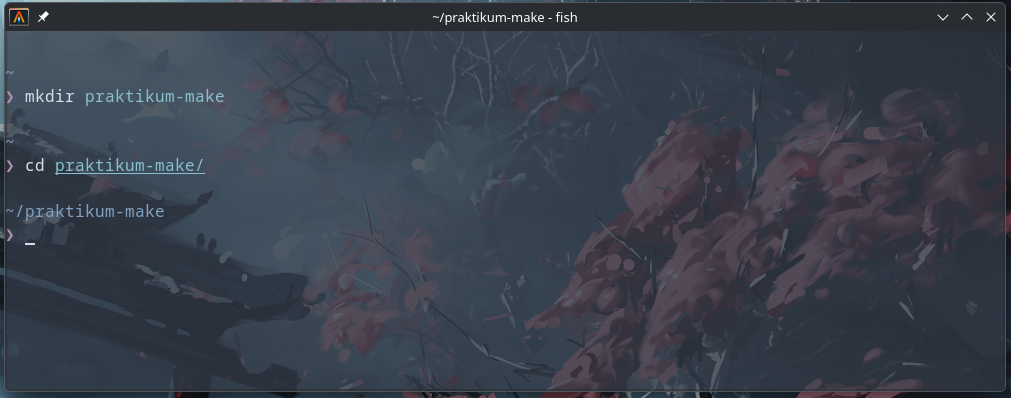
\includegraphics[width=0.75\textwidth]{Figure/06/direktori-make.png}
    \caption{Direktori Kerja Praktikum Modul 6}
    \label{fig:m06-direktori}
\end{figure}
    \item Pastikan instrumen penunjang \texttt{make} terdeteksi di dalam sistem.
    \begin{lstlisting}[language=bash, caption={Mengecek versi Make}]
make --version
    \end{lstlisting}
    \begin{figure}[H]
    \centering
    % TODO: ganti dengan screenshot hasil praktikum
    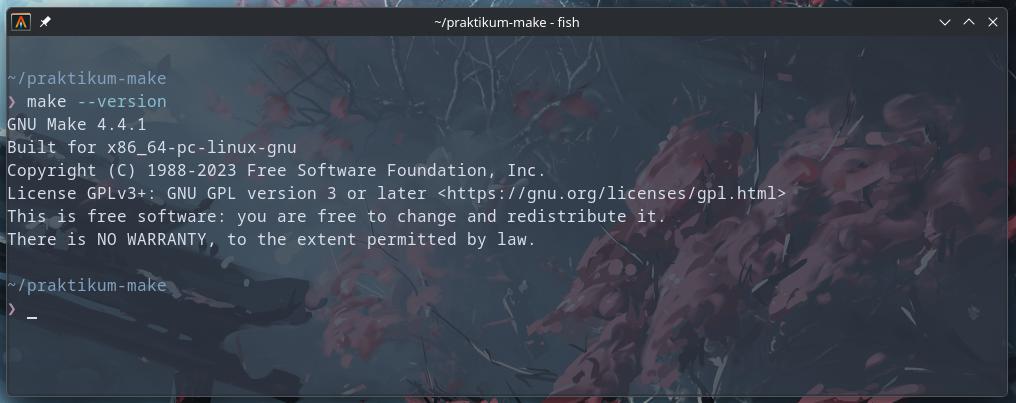
\includegraphics[width=0.75\textwidth]{Figure/06/make-version.png}
    \caption{Validasi Instalasi Make}
    \label{fig:m06-make-version}
\end{figure}

    Jika terminal menampilkan versi rilis (seperti \textit{GNU Make 4.4.1} dsb), Anda siap untuk mendaki ke tahap berikutnya.
\end{enumerate}

\subsection{Sesi 1: Penulisan Makefile Mendasar}
\label{sec:m06-sesi-1}
Di sesi ini, Anda akan memandu kompilasi sebuah kode program C tunggal menggunakan instruksi yang diletakkan dalam berkas \texttt{Makefile}.

\begin{enumerate}
    \item Gunakan editor teks \texttt{nano} untuk menulis berkas program C sederhana. Ketik instruksi ini di terminal:
    \begin{lstlisting}[language=bash, caption={Membuka nano untuk berkas hello.c}]
nano hello.c
    \end{lstlisting}
    Lalu ketik baris berikut ini:
    \begin{lstlisting}[language=c, caption={Isi file hello.c}]
#include <stdio.h>
int main() {
    printf("Ajaib! Program ini dikompilasi oleh Make!\n");
    return 0;
}
    \end{lstlisting}
    \textit{Untuk menyimpan: Tekan dan tahan tombol \textbf{Ctrl}, lalu tekan \textbf{O} (huruf O). Setelah pesan "File Name to Write" di bawah muncul, pencet \textbf{Enter}.}\\
    \textit{Untuk keluar: Tekan \textbf{Ctrl+X}.}

    \begin{figure}[H]
    \centering
    % TODO: ganti dengan screenshot hasil praktikum
    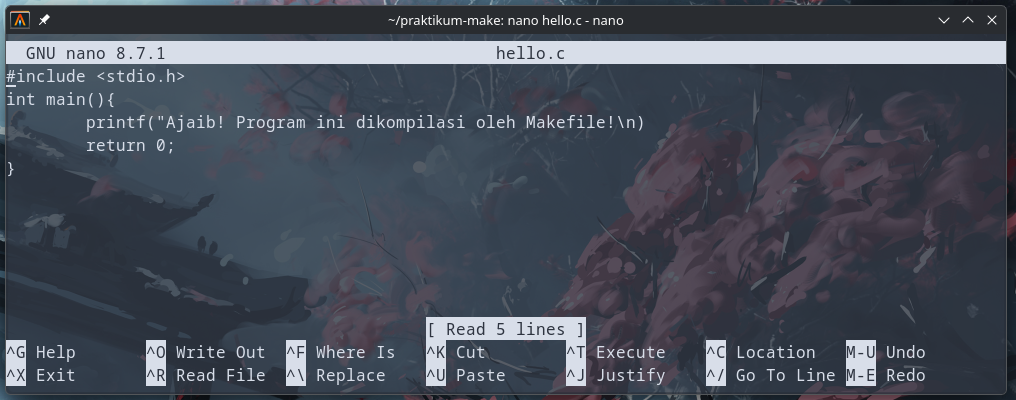
\includegraphics[width=0.75\textwidth]{Figure/06/hello-c.png}
    \caption{Membuat File hello.c dengan Nano}
    \label{fig:m06-hello-c}
\end{figure}

    \item Sekarang, buat instrumen pusat kita, yaitu berkas \texttt{Makefile}. Ingat, huruf 'M' harus dikapitalisasi. Jalankan:
    \begin{lstlisting}[language=bash, caption={Ketik ini di terminal}]
nano Makefile
    \end{lstlisting}

    \item Salin baris berikut. \textbf{SANGAT PENTING:} Di baris ke-2 persis sebelum kursor menyentuh huruf g pada kata `gcc`, Anda TIDAK BOLEH memencet tombol SPASI untuk menjorokkan teks, Anda HARUS MEMENCET TOMBOL \textbf{TAB} (biasanya berada di atas tombol \textit{Caps Lock}). Make sangat ketat terkait aturan penulisan spasi!
    
    \begin{lstlisting}[language=make, caption={Makefile dasar}]
program-halo: hello.c
	gcc hello.c -o program-halo
    \end{lstlisting}
    \textit{Simpan file ini (Ctrl+O, Enter) dan kelur dari nano (Ctrl+X).}

    \begin{figure}[H]
        \centering
        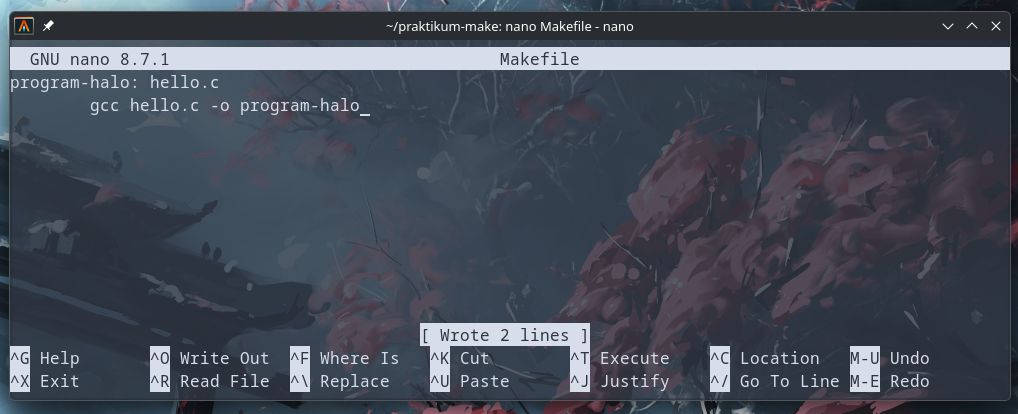
\includegraphics[width=0.75\textwidth]{Figure/06/make.png}
        \caption{Isi Makefile untuk Sesi 1}
        \label{fig:m06-makefile-sesi1}
    \end{figure}


    \item Untuk menginstruksikan \textit{Make} menjalankan target, Anda hanya cukup memanggil \verb|make| tanpa atribut di konsol. 
    \begin{lstlisting}[language=bash, caption={Eksekusi Makefile}]
make
    \end{lstlisting}

    \begin{figure}[H]
        \centering
        
\includegraphics[width=0.75\textwidth]{Figure/06/make-compile.png}
        \caption{Hasil compile dengan Make}
        \label{fig:m06-make-compile}
    \end{figure}

    Perhatikan bahwa \textit{Make} secara otomatis memantulkan perintah `\texttt{gcc hello.c -o program-halo}` ke konsol dan program tersebut telah selesai dikompilasi! Anda dapat membuktikannya dan langsung menjalankannya lewat instruksi:
    \begin{lstlisting}[language=bash, caption={Menjalankan target}]
./program-halo
    \end{lstlisting}

    \begin{figure}[H]
        \centering
        
\includegraphics[width=0.75\textwidth]{Figure/06/make-execute.png}
        \caption{Hasil Eksekusi Target program-halo}
        \label{fig:m06-make-execute}
    \end{figure}

    \item Coba jalankan \verb|make| sekali lagi.
    \begin{lstlisting}[language=bash, caption={Jalankan instruksi ini lagi}]
make
    \end{lstlisting}
    Anda akan mendapatkan pesan seperti \textbf{"make: 'program-halo' is up to date"}. Alasan ini adalah inti utama Makefile: Ia mengecek bahwa \texttt{hello.c} (syarat) tidak mengalami perubahan (misalnya kita belum mengeditnya) sejak terakhir kali \texttt{program-halo} (target) dicetak. Karena isinya stabil, \textit{Make} enggan membuang-buang daya waktu dan komputasi!
\end{enumerate}

\begin{figure}[H]
    \centering
    % TODO: ganti dengan screenshot hasil praktikum
    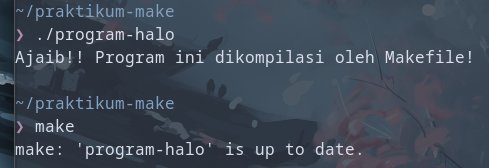
\includegraphics[width=0.75\textwidth]{Figure/06/make-compile-2.png}
    \caption{Hasil Eksekusi dan validasi up-to-date Make}
    \label{fig:m06-make-compile-2}
\end{figure}

\subsection{Sesi 2: Target Kompleks dan Pengunaan Variabel Otomatis}
\label{sec:m06-sesi-2}
Di sesi lanjutan ini, kita akan mereplikasi gaya perakitan berkas asli program-program profesional. Makefile Anda akan merangkum bermacam berkas, membungkus perintah kompilasi ke dalam Variabel Makro, dan mendefinisikan sebuah target baru \texttt{clean} guna membuang sampah file hasil.

\begin{enumerate}
    \item Mari kita buat dua berkas C, satu perpustakaan (`.h`), satu turunan (`.c`), dan satu fungsi gerbang pusar (`.c`).

    \textbf{Bagian 1: Matematika.h}\\
    Jalankan: \texttt{nano matematika.h}
    \begin{lstlisting}[language=c, caption={Isi matematika.h}]
int kali(int x, int y);
    \end{lstlisting}
    \textit{Simpan dan Keluar. (Ctrl+O, Enter $\rightarrow$ Ctrl+X)}

    \begin{figure}[H]
        \centering
        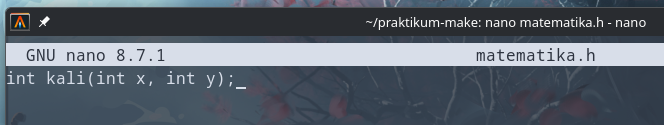
\includegraphics[width=0.75\textwidth]{Figure/06/matematika-h.png}
        \caption{Membuat File matematika.h dengan Nano}
        \label{fig:m06-matematika-h}
    \end{figure}

    \textbf{Bagian 2: Matematika.c}\\
    Jalankan: \texttt{nano matematika.c}
    \begin{lstlisting}[language=c, caption={Isi matematika.c}]
#include "matematika.h"
int kali(int x, int y){
    return x * y;
}
    \end{lstlisting}
    \textit{Simpan dan Keluar. (Ctrl+O, Enter $\rightarrow$ Ctrl+X)}

    \begin{figure}[H]
        \centering
        
\includegraphics[width=0.75\textwidth]{Figure/06/matematika-c.png}
        \caption{Membuat File matematika.c dengan Nano}
        \label{fig:m06-matematika-c}
    \end{figure}

    \textbf{Bagian 3: Main.c}\\
    Jalankan: \texttt{nano main.c}
    \begin{lstlisting}[language=c, caption={Isi main.c}]
#include <stdio.h>
#include "matematika.h"

int main() {
    printf("Hasil dari 6 dikali 7 adalah: %d\n", kali(6, 7));
    return 0;
}
    \end{lstlisting}
    \textit{Simpan dan Keluar. (Ctrl+O, Enter $\rightarrow$ Ctrl+X)}

    \begin{figure}[H]
        \centering
        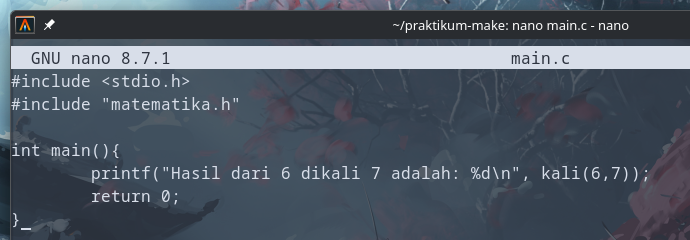
\includegraphics[width=0.75\textwidth]{Figure/06/main-c.png}
        \caption{Membuat File main.c dengan Nano}
        \label{fig:m06-main-c}
    \end{figure}

    \item Sekarang, hapus/timpa isi `Makefile` lama kita sebelumnya dan gunakan skrip utuh canggih berikut.\\
    Jalankan: \texttt{nano Makefile}, kemudian copot/hapus isinya lalu ganti menjadi ini.\\
    \textbf{Pengingat Jarak TAB:} Pastikan untuk setiap lajur baru \textit{Recipe/Perintah terminal} di bawah tulisan berawalan tab, yakni tepatnya berada pada awal baris ke-6 dan ke-9 di bawah ini mengandalkan tombol \lstinline{<TAB>}.

    \begin{lstlisting}[language=make, caption={Makefile Lanjut dengan Macro dan Target}]
CC = gcc
CFLAGS = -Wall

# "$^" bermagnitudo semua prerequisites, "$@" adalah Target yaitu 'aplikasi'
aplikasi: main.c matematika.c
	$(CC) $(CFLAGS) $^ -o $@

# Perintah clean akan merestorasi folder kerja menjadi rapi
clean:
	rm -f aplikasi *.o
    \end{lstlisting}
    \textit{Simpan dan Keluar. (Ctrl+O, Enter $\rightarrow$ Ctrl+X)}

    \begin{figure}[H]
        \centering
        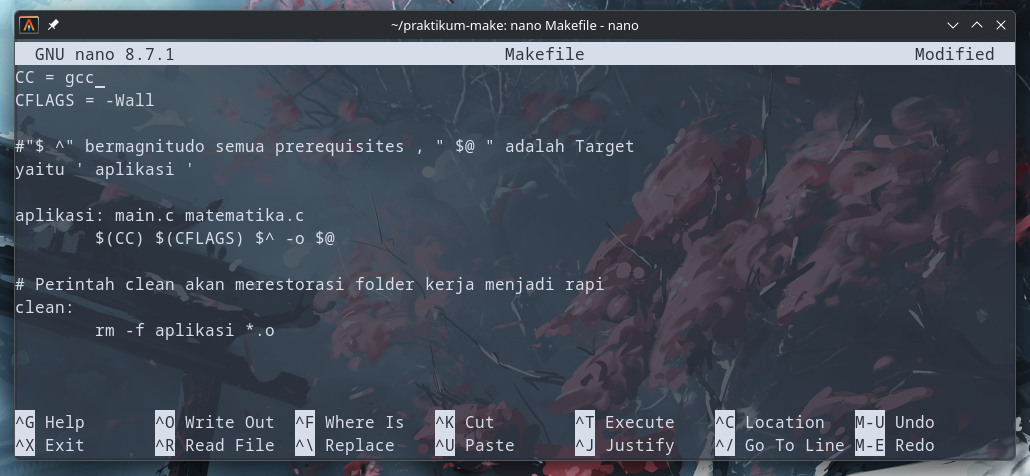
\includegraphics[width=0.75\textwidth]{Figure/06/new-makefile.png}
        \caption{Isi Makefile untuk Sesi 2}
        \label{fig:m06-new-makefile}
    \end{figure}
        

    \item Jalankan proses \textit{Make} yang sekarang akan mendeteksi prasyarat `\texttt{aplikasi}`.
    \begin{lstlisting}[language=bash, caption={Menjalankan multi-file Make}]
make
./aplikasi
    \end{lstlisting}
    Anda akan melihat bahwa Make secara otomatis mengompilasi `main.c` dan `matematika.c` menjadi `aplikasi`, lalu menjalankannya untuk menampilkan hasil perkalian 6 dan 7.
    \begin{figure}[H]
        \centering
        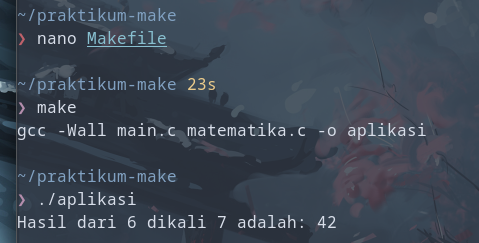
\includegraphics[width=0.75\textwidth]{Figure/06/make-compile-3.png}
        \caption{Hasil Eksekusi Target aplikasi}
        \label{fig:m06-make-compile-3}
    \end{figure}

    \item Terakhir, panggil perintah target buatan Anda untuk mengkandaskan/membersihkan file executable sisa sehingga ruang kerja kembali murni hanya berisi \textit{source code} C saja.
    \begin{lstlisting}[language=bash, caption={Merobohkan file hasil eksekusi}]
make clean
ls
    \end{lstlisting}
    Lihat bagaimana \texttt{ls} kini tidak lagi memampangkan target \texttt{aplikasi} berwarna hijau; Ia telah ludes dan aman dari sisa jejak!
\end{enumerate}

\begin{figure}[H]
    \centering
    \begin{subfigure}[b]{0.45\textwidth}
        \centering
        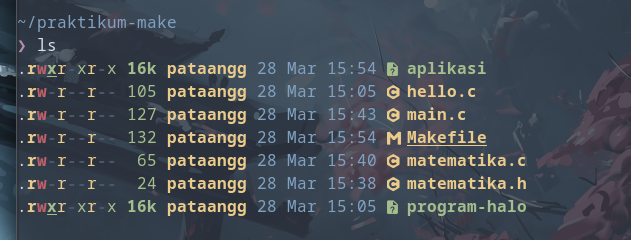
\includegraphics[width=\textwidth]{Figure/06/before-make-clean.png}
        \caption{Sebelum menjalankan \texttt{make clean}}
        \label{fig:m06-before-clean}
    \end{subfigure}
    \hfill
    \begin{subfigure}[b]{0.45\textwidth}
        \centering
        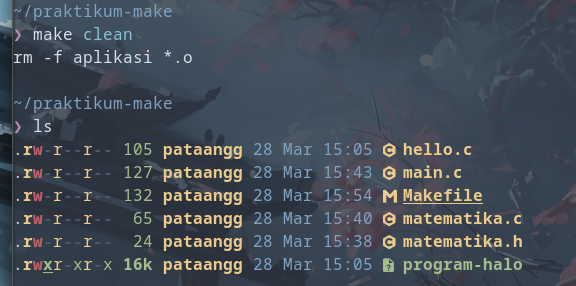
\includegraphics[width=\textwidth]{Figure/06/after-make-clean.png}
        \caption{Setelah menjalankan \texttt{make clean}}
        \label{fig:m06-after-clean}
    \end{subfigure}
    \caption{Perbandingan Direktori Sebelum dan Sesudah Target \texttt{clean} di Makefile}
    \label{fig:m06-make-clean-comparison}
\end{figure}


% --- Tugas mandiri ---
\newpage
\section{Hands-On}
\label{sec:m06-hands-on}

Pada sesi Hands-On ini, Anda akan diminta untuk menggabungkan pengetahuan dari \textbf{Modul 5 (Sistem Build dengan GCC) dan Modul 6 (Otomatisasi dengan Makefile)}. Anda akan membangun sebuah program kalkulator modular sederhana. Buktikan setiap langkah yang Anda lakukan dengan \textit{screenshot} terminal.

\subsection{Tugas 1: Persiapan File Kode Sumber (C)}
\begin{enumerate}
    \item Buatlah sebuah direktori baru bernama \texttt{tugas-kalkulator} dan masuk ke dalamnya.
    \item Buatlah tiga buah file C menggunakan \texttt{nano}:
    \begin{itemize}
        \item \textbf{\texttt{kalkulator.h}} : Berisi deklarasi dua fungsi: \texttt{tambah(int a, int b)} dan \texttt{kurang(int a, int b)}.
        \item \textbf{\texttt{kalkulator.c}} : Berisi implementasi/isi dari fungsi \texttt{tambah} dan \texttt{kurang} tersebut.
        \item \textbf{\texttt{utama.c}} : Berisi fungsi \texttt{main()} yang memanggil fungsi \texttt{tambah(10, 5)} dan \texttt{kurang(10, 5)} lalu mencetak hasilnya ke layar menggunakan \texttt{printf}. Jangan lupa melakukan \texttt{\#include "kalkulator.h"}.
    \end{itemize}
    \item \textbf{Bukti:} Sertakan \textbf{screenshot} kode sumber dari ketiga file tersebut menggunakan perintah \texttt{cat nama\_file}.
\end{enumerate}

\subsection{Tugas 2: Kompilasi Manual dengan GCC (Review Modul 5)}
\begin{enumerate}
    \item Lakukan tahapan kompilasi secara merinci untuk file \texttt{utama.c} dan \texttt{kalkulator.c} hingga menjadi file objek (\texttt{.o}) menggunakan flag \texttt{-c}.
    \item Gabungkan (Link) kedua file objek tersebut (\texttt{utama.o} dan \texttt{kalkulator.o}) menjadi sebuah \textit{executable} utuh bernama \texttt{kalkulator-manual}.
    \item Jalankan \texttt{./kalkulator-manual} untuk memastikan program berjalan dengan benar.
    \item \textbf{Bukti:} Sertakan \textbf{screenshot} perintah-perintah kompilasi GCC tersebut beserta hasil eksekusi programnya.
\end{enumerate}

\subsection{Tugas 3: Mengotomatisasi dengan Makefile (Review Modul 6)}
\begin{enumerate}
    \item Hapus file objek (\texttt{.o}) dan aplikasi *executable* (\texttt{kalkulator-manual}) yang telah Anda buat pada Tugas 2 secara manual (menggunakan perintah \texttt{rm}).
    \item Buatlah sebuah berkas \texttt{Makefile} untuk mengotomatisasi proses pada Tugas 2. 
    \item Pastikan \texttt{Makefile} tersebut memiliki:
    \begin{itemize}
        \item Variabel \texttt{CC} untuk \texttt{gcc}.
        \item Variabel \texttt{CFLAGS} yang minimal berisi \texttt{-Wall}.
        \item Target utama bernama \texttt{kalkulator-otomatis} bermagnitudo dependensi/syarat dari kode C yang Anda buat.
        \item Target \texttt{clean} untuk membersihkan folder kerja dari file \texttt{.o} dan program \textit{executable}.
    \end{itemize}
    \item Jalankan perintah \texttt{make}. Tunjukkan bahwa program berhasil dikompilasi secara otomatis.
    \item Jalankan perintah \texttt{make clean}. Tunjukkan melalui perintah \texttt{ls} bahwa folder kerja Anda kembali bersih.
    \item \textbf{Bukti:} Sertakan \textbf{screenshot} isi \texttt{Makefile} Anda (gunakan \texttt{cat Makefile}), \textbf{screenshot} eksekusi \texttt{make} dan hasil jalannya program, serta \textbf{screenshot} eksekusi \texttt{make clean} dengan bukti folder kembali bersih (\texttt{ls}).
\end{enumerate}
% % ============================================================
%  Modul 7 — Booting dan Framework Sistem Operasi
% ============================================================

\chapter{Booting dan Framework Sistem Operasi}
\label{chap:modul-07}

% --- 1. Tujuan dan Output Praktikum ---
\section{Tujuan dan Output Praktikum}

\subsection{Tujuan Praktikum}
Setelah menyelesaikan praktikum ini, mahasiswa diharapkan mampu:
\begin{enumerate}
    \item Memahami konsep proses \textit{booting} beserta fungsi komponen penyusun kerangka dasar sistem operasi (seperti \textit{Multiboot Header}, algoritma C/Assembly, dan \textit{Linker Script}).
    \item Melakukan proses perakitan (\textit{build}) melalui kompilasi silang (\textit{cross-compilation}) berbasis kontainer terisolasi serta menyimulasikan peluncuran sistem operasinya secara aman menggunakan emulator QEMU.
\end{enumerate}

\subsection{Output Praktikum}
Pada akhir praktikum ini, mahasiswa diharapkan menghasilkan:
\begin{itemize}
    \item Penjelasan analitis mengenai fungsi dari masing-masing berkas penyusun arsitektur sistem operasi (terutama \texttt{boot.asm}, \texttt{kernel.c}, dan \texttt{linker.ld}).
    \item Berkas instalasi sistem operasi berformat \texttt{.iso} yang berhasil ter-\textit{compile} dan mematuhi spesifikasi standar \textit{bootloader}, beserta tangkapan layar (\textit{screenshot}) bukti sistem sukses melewati siklus \textit{booting} di dalam peramban QEMU.
\end{itemize}

% --- 2. Dasar Teori ---
\newpage
\section{Dasar Teori}

\subsection{Pengenalan OS Framework dan Booting}
Sistem operasi adalah perangkat lunak utama yang berinteraksi langsung dengan fisik perangkat keras komputer \cite{Silberschatz2018}. Saat komputer pertama kali dinyalakan, serangkaian instruksi berurutan yang disebut \textit{booting} akan berjalan. Proses ini diibaratkan seperti lari estafet; satu program berukuran kecil akan memanggil program lain yang ukurannya sedikit lebih besar, berlanjut terus hingga sistem operasi secara utuh berhasil mengambil alih kendali komputer.

\begin{figure}[h]
    \centering
    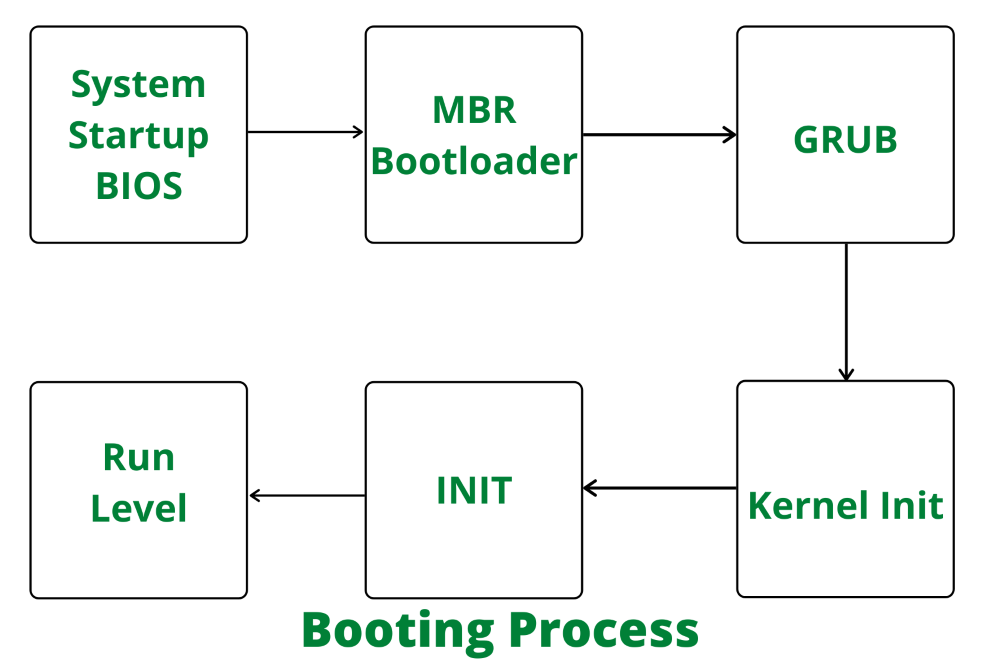
\includegraphics[width=0.75\textwidth]{Figure/07/1.png}
    \caption{Visualisasi proses booting komputer secara berurutan}
    \label{fig:m07-boot-sequence}
\end{figure}

Berdasarkan ilustrasi diagram pada Gambar \ref{fig:m07-boot-sequence}, tahapan \textit{booting} secara umum dapat dijabarkan menjadi 6 langkah sederhana:
\begin{enumerate}
    \item \textbf{System Startup BIOS}: Saat tombol \textit{power} ditekan, komputer akan menjalankan program bawaan mesin bernama BIOS. BIOS bertugas mengecek apakah komponen fisik (seperti RAM dan \textit{keyboard}) sudah berfungsi normal.
    \item \textbf{MBR Bootloader}: Setelah fisik dipastikan aman, BIOS akan mencari instruksi pertama di ujung memori penyimpanan (disk) yang lokasinya disebut MBR. MBR ibarat pintu masuk menuju program selanjutnya.
    \item \textbf{GRUB}: MBR kemudian memanggil program pengelola \textit{boot} yang lebih pintar, salah satunya adalah GRUB. GRUB inilah yang tahu persis di mana sistem operasi kita berada, lalu memuatnya ke memori utama (RAM).
    \item \textbf{Kernel Init}: Setelah dimuat ke RAM, inti dari sistem operasi (disebut \textit{Kernel}) mulai terbangun. Kernel secara resmi mengambil alih kendali komputer sepenuhnya dari tangan GRUB.
    \item \textbf{INIT}: Kernel kemudian menyalakan satu proses utama penggerak yang disebut \texttt{INIT}. Proses \texttt{INIT} inilah yang bertugas membangunkan fitur-fitur maupun layanan pendukung lain di dalam OS.
    \item \textbf{Run Level}: Ini adalah kondisi garis finis. Pada tahap \textit{Run Level}, komputer sudah "sadar" sepenuhnya (misalnya berhasil masuk ke layar Terminal/Desktop) dan siap menerima interaksi dari pengguna.
\end{enumerate}

\subsection{Kernel Bare-Bones dan Spesifikasi Multiboot}
Mengembangkan sistem operasi mensyaratkan kerangka dasar (\textit{bare-bones}) yang dapat beroperasi tanpa dukungan sistem operasi lain \cite{osdev_wiki_barebones}. Karena berstatus independen dan tidak menggunakan modul fungsi dari \textit{standard library}, inisialisasi awal pada perangkat keras komputer wajib diserahkan kepada komponen antarmuka yang sangat spesifik.

\subsubsection{Standar Multiboot pada Bootloader}
Agar perangkat \textit{bootloader} utama (seperti GRUB) bersedia menemukan dan memuat kernel spesifik OS ke dalam memori, kerangka OS didesain wajib mematuhi ketentuan dari \textbf{Spesifikasi Multiboot} (GNU). Berdasarkan spesifikasi instruksi ini, berkas kompilasi biner awal harus menyuntikkan deklarasi \textit{Multiboot Header} di bagian awal blok \textit{header} berkas (\textit{file format}). 

Tanda \textit{header} perizinan ini ditulis menggunakan bahasa Assembly (sebagaimana dideklarasikan melalui \texttt{boot.asm}) dengan menyertakan \textit{magic number} unik berbasis bilangan heksadesimal bernilai tetap (\texttt{0x1BADB002}) \cite{gnu_multiboot}. Kehadiran nomor ajaib ini menjadi patokan (\textit{signature}) identifikasi GRUB untuk mengenalinya sebagai OS terstandarisasi, sebelum perannya meredup dan mengandalkan proses siklus selanjutnya pada fungsi \texttt{main()} program bahasa terapan C (\texttt{kernel.c}).

\subsubsection{Manajemen Relokasi dengan Linker Script}
Pada arsitektur OS \textit{bare-metal}, penetapan perihal letak tatanan alamat memori tidak ditangani \textit{loader} dinamis. Ketiadaan itu mensyaratkan eksistensi berkas \textit{Linker Script} (\texttt{linker.ld}) untuk secara tegas mendikte alokasi perpindahan posisi kode memori \cite{bryant2015computer}. Pada sistem berbasis arsitektur x86, kernel OS umumnya diamanatkan agar diload ke ruang memori fisik minimal berawal di unit \texttt{1M} (\texttt{0x100000}), membiarkan ruang memori di bawah 1MB tetap diakses eksklusif sebagai alokasi sakral konfigurasi antarmuka untuk BIOS (\textit{Basic Input/Output System}) maupun Vesa-Graphic peranti tampilan visual perangkat.

\subsection{Simulasi Perangkat Keras melalui QEMU}
Setelah semua bagian kode dipersatukan menjadi satu format instalasi kepingan siap-boot (\texttt{os.iso}), eksekusi \textit{host-machine} pada komputer secara telanjang patut dihindari. Komputasi pengujian OS sangat sarat atas probabilitas kekacauan yang sanggup merusak alur partisi (*storage*) mesin \textit{host} sesungguhnya.

Keseluruhan perancangan diuji mutlak dalam isolasi peranti \textbf{QEMU}. Emulator x86 ini membentangkan platform simulasi lengkap mulai dari abstraksi CPU, register internal, kepingan Random Access Memory, hingga konfigurasi Serial-Port. Pemanfaatan QEMU menjadi prasyarat esensial guna mengekstrak pantauan alur \textit{log-sequence} operasi komputasi saat prosedur (\textit{Booting}) terjadi dari menit paling awal secara transparan, serta memudahkan rekam jejak apabila fungsi sinkronisasi (seperti penentuan jadwal \textit{task-scheduler}) menuai kecacatan algoritma teknis (*Crash-Faults*).

Tabel \ref{tab:m07-dasar-teori} merangkum hal-hal penting agar pembentukan konsep di atas lebih mudah ditinjau di modul ini.

\newpage
\begin{table}[!ht]
\caption{Tabel Ringkasan Dasar Teori}
\label{tab:m07-dasar-teori}
\centering
\begin{tabulary}{\textwidth}{|L|L|}
\hline
\textbf{Konsep / Tools} & \textbf{Penjelasan Singkat} \\ \hline
Bootloader (GRUB) & Program di sektor awal mesin yang membaca aturan GNU Multiboot dan membangunkan CPU arsitektur 32-bit. \\ \hline
\texttt{boot.asm} & Program instruksi mesin (\textit{Assembly}) bervolume hemat yang merengkuh (\textit{Entry-Point}) izin kendali booting OS. \\ \hline
Linker Script (\texttt{linker.ld}) & Merupakan set aturan logis tata letak posisi kode memori spesifik di RAM kernel (contoh blok: \texttt{0x100000}). \\ \hline
Multiboot Magic Number & Penanda (\textit{signature}) biner wajib penyuntingan GNU untuk menyatakan bahwa berkas bersangkutan diakui Bootloader. \\ \hline
QEMU & Sebuah perangkat lunak berbasis \textit{emulator} mandiri nan aman membedah pengujian alur OS instrumen format .iso. \\ \hline
\end{tabulary}
\end{table}

% --- 3. Alat dan Bahan ---
\newpage
\section{Alat dan Bahan}
\label{sec:m07-alat-bahan}

\subsection{Perangkat Keras}
\begin{itemize}
    \item PC atau Laptop dengan arsitektur prosesor x86/x64.
    \item Memori minimal 4GB RAM dan kapasitas penyimpanan sekunder yang memadai.
\end{itemize}

\subsection{Perangkat Lunak (Bahan Praktikum)}
\begin{itemize}
    \item Sistem operasi \textit{host} (Windows, Linux, atau macOS).
    \item Text Editor atau IDE (misalnya Visual Studio Code).
    \item Docker (Docker Desktop atau Docker Engine) untuk proses kompilasi (\textit{cross-compiling}) di lingkungan terisolasi.
    \item QEMU Emulator (khususnya paket \texttt{qemu-system-i386} atau \texttt{qemu-system-x86\_64}) sebagai mesin virtual.
    \item Paket kode dasar praktikum (\textit{Starter Code OS 32-bit}) yang dikloning/diunduh dari repositori GitHub: \url{https://github.com/Aziz097/starter-code-os32}.
\end{itemize}

% --- 4. Langkah-Langkah Praktikum ---
\newpage
\section{Langkah-Langkah Praktikum}

\subsection{Persiapan 1: Instalasi Dependensi Dasar dan Docker}
\label{sec:m07-persiapan-install}
Sebelum mengolah \textit{image}, Anda perlu memasang pustaka pengembangan (\textit{multilib compiler}, QEMU, dsb) serta \textit{engine} Docker di mesin \textit{host} utama Anda (khususnya untuk pengguna lingkungan basis distribusi Ubuntu/Debian).
\begin{enumerate}
    \item Buka Terminal dan perbarui indeks \textit{repository}, lalu pasang dependensi \textit{cross-compile} x86 dan QEMU:
    \begin{lstlisting}[language=bash, caption={Instalasi pustaka dasar dan perangkat virtual QEMU}]
sudo apt update
sudo apt install -y build-essential gcc-multilib nasm \
                    qemu-system-x86 grub-pc-bin xorriso
    \end{lstlisting}
    \item Selanjutnya, pastikan Docker terpasang di sistem. Jika belum, instal Docker Engine:
    \begin{lstlisting}[language=bash, caption={Instalasi Docker Engine}]
sudo apt install -y docker.io
    \end{lstlisting}
    \item (Opsional namun disarankan) Tambahkan \textit{user} Anda ke grup \texttt{docker} agar kelak terbebas dari awalan \texttt{sudo} ketika mengeksekusi komando Docker.
    \begin{lstlisting}[language=bash, caption={Konfigurasi hak otorisasi akses pengguna Docker}]
sudo usermod -aG docker $USER
    \end{lstlisting}
    \textit{Catatan: \textit{Restart} atau \textit{relog} Terminal Anda agar perubahan perizinan grup ini langsung terbaca.}
\end{enumerate}

\subsection{Persiapan 2: Menjalankan Mesin Terisolasi}
\label{sec:m07-persiapan-env}
Langkah ini menyiapkan ruang kerja terisolasi agar \textit{tools} kompilasi dan dependensi sistem operasi tidak mengotori mesin \textit{host} (laptop) Anda.
\begin{enumerate}
    \item Buka terminal, pastikan posisi Anda sudah berada di dalam folder proyek \texttt{starter-code-os32-main}, lalu terjun ke mode simulasi lingkungan dengan mengeksekusi \textit{script runner}-nya:
    \begin{lstlisting}[language=bash, caption={Perintah meluncurkan container Docker}]
# Di sistem Windows (menggunakan Git Bash/WSL) atau Linux/macOS:
./run-docker.sh
    \end{lstlisting}
    
    \begin{figure}[!ht]
        \centering
        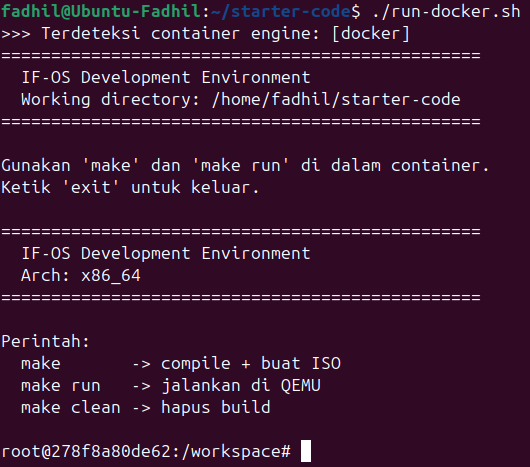
\includegraphics[width=0.85\textwidth]{Figure/07/8.png}
        \caption{Terminal masuk secara interaktif dengan indikator berpindahnya ruang kendali menjadi status \texttt{root@...:/workspace\#} di dalam kontainer \texttt{ifos-dev}}
        \label{fig:m07-docker-masuk}
    \end{figure}

    \item Skrip tersebut akan merakit atau menarik (\textit{pull}) peranti kontainer secara otomatis, ditandai dari tampilan baris \textit{working directory} Anda.
\end{enumerate}

\subsection{Sesi 1: Kompilasi Biner OS (Make)}
\label{sec:m07-sesi-1}
Di dalam lingkungan terisolasi ini, Anda akan menjahit (\textit{linking}) susunan berkas instruksi Assembly (\texttt{boot.asm}) dan C (\texttt{kernel.c}) menjadi satu \textit{file} instalasi terpadu (\texttt{os.iso}).
\begin{enumerate}
    \item Di dalam \textit{shell} kontainer Docker, periksa isi folder kerja menggunakan perintah \texttt{ls}. Secara mendasar, \textit{folder} ini adalah pantulan sikronisasi repositori Anda di mesin \textit{host} Anda.
    \item Lakukan kompilasi kode biner sumber dan menautkannya ke instruksi Multiboot GRUB melalui otomasi perintah sistem \texttt{make}:
    \begin{lstlisting}[language=bash, caption={Perintah kompilasi berkas instruksi OS}]
make
    \end{lstlisting}

    \begin{figure}[!ht]
        \centering
        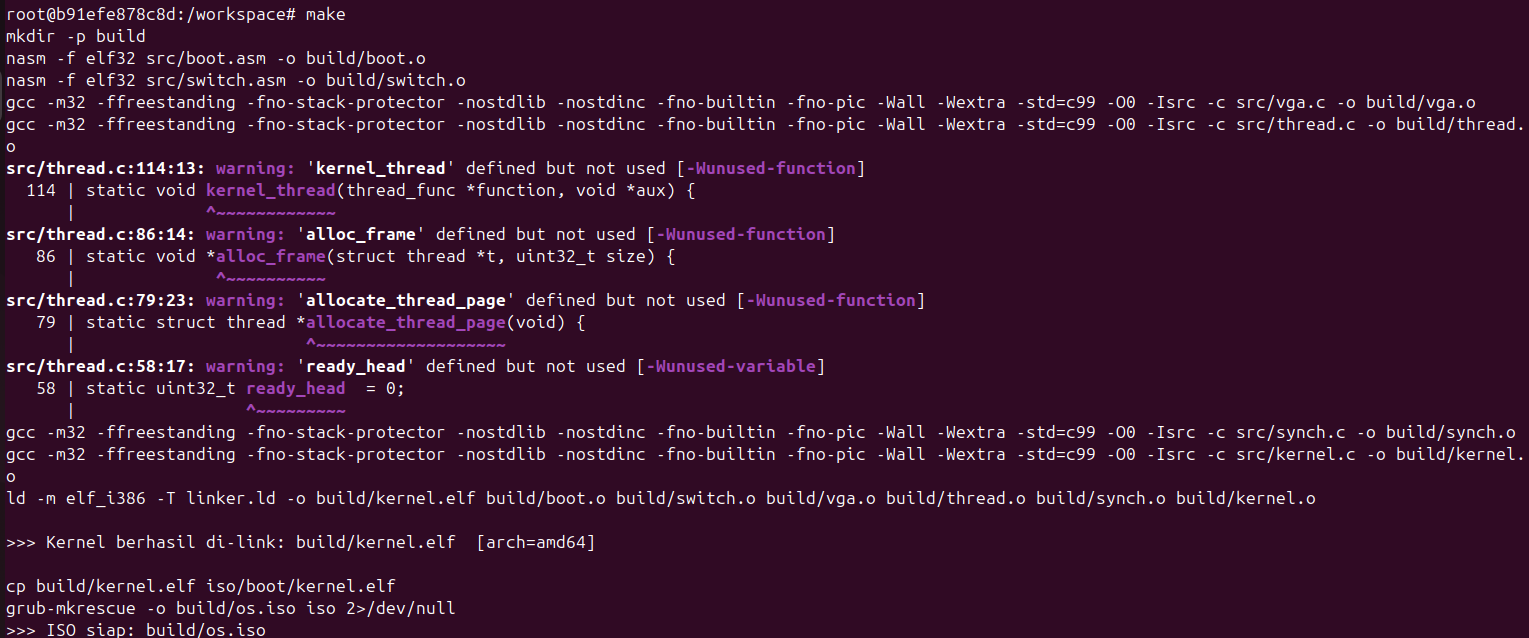
\includegraphics[width=0.9\textwidth]{Figure/07/9.png}
        \caption{Laporan suksesnya perintah \textit{make} pada \textit{shell} menautkan objek program C hingga \textit{linker} GRUB biner \texttt{os.iso}}
        \label{fig:m07-make-success}
    \end{figure}
    
    \item Perhatikan teks keluaran (\textit{output}) kompilator. Jika urutan berhasil, fungsi-fungsi instruksi selesai diproses dan Anda mendapat validasi bertuliskan: \texttt{>>> ISO siap: build/os.iso}.
\end{enumerate}

\subsection{Sesi 2: Eksekusi dan Verifikasi di QEMU}
\label{sec:m07-sesi-2}
Tahapan penutup modul ini adalah menguji coba berkas \textit{bare-metal} OS \texttt{.iso} tersebut ke dalam peranti simulator \textit{hardware} berarsitektur x86 bernama emulator QEMU.
\begin{enumerate}
    \item Keluar dari terminal kontainer Docker (dengan mengetik \texttt{exit}) atau buka jendela Terminal baru di mesin \textit{host} asli Anda. Pastikan posisi direktori Anda berada di folder proyek \texttt{starter-code-os32-main}.
    \item Laksanakan tes pembuka eksekusi skrip emulator dengan menjalankan perintah \textit{make} berikut di mesin \textit{host} Anda (yang sudah diinstal QEMU pada Persiapan 1):
    \begin{lstlisting}[language=bash, caption={Perintah memacu virtualisasi QEMU meluncurkan file OS biner}]
make run
    \end{lstlisting}

    \item Jendela layar QEMU (atau konsol emulator) akan muncul dan mengambil alih tampilan dengan antarmuka \textit{Bootloader} fiktif GRUB. \textit{Kernel loader} selanjutnya akan dipandu masuk melalui proses *booting* riil ke antarmuka utama sistem operasi.
    
    \item Oleh karena fitur fungsional komputasi \textit{Thread Scheduling} saat ini masih dirancang kosong secara alur \textit{stub} dalam struktur inti \textit{source code}, wajar apabila OS mencetak log luaran yang bermuara tertahan akibat pesan peringatan berikut (menandakan skema \textit{booting} sudah berhasil dimuat secara mulus):
    \begin{lstlisting}[caption={Pesan luaran *Thread block* sebagai bukti akhir keberhasilan simulasi di QEMU}]
===================================
  IF-OS  |  Praktikum Sistem Operasi
===================================

Inisialisasi sistem thread...
Membuat thread A, B, C...
Memulai scheduling...

ERROR: kernel_main() kembali dari thread_block()!
    \end{lstlisting}
\end{enumerate}

% % ============================================================
%  Modul 8 — Implementasi Multi-threading
% ============================================================

\chapter{Implementasi Multi-threading}
\label{chap:modul-08}

% --- 1. Tujuan dan Output Praktikum ---
\section{Tujuan dan Output Praktikum}

\subsection{Tujuan Praktikum}
Tujuan yang diharapkan dapat dicapai oleh mahasiswa adalah:
\begin{enumerate}
    \item Memahami arsitektur perangkat lunak dalam manajemen \textit{thread} (termasuk abstraksi \textit{Thread Control Block}) dan algoritma penjadwalan (\textit{scheduling}) pada tingkat inti sistem operasi (\textit{kernel-level}).
    \item Mempraktikkan implementasi logika \textit{Context Switching} untuk memfasilitasi eksekusi \textit{multi-threading} melalui penyimpanan dan pemuatan status register CPU (memanfaatkan manipulasi bahasa tingkat rendah/Assembly).
\end{enumerate}

\subsection{Output Praktikum}
Hasil luaran yang diekspektasikan adalah kelengkapan instrumen berikut:
\begin{itemize}
    \item Implementasi fungsional dari modifikasi berkas sumber (khususnya penyesuaian pada logika \texttt{thread.c}, \texttt{switch.asm}, dan \texttt{scheduler.h}) yang terbukti mampu mengompilasi rekayasa antrean \textit{thread}.
    \item Tangkapan layar (\textit{screenshot}) keluaran terminal dari emulator QEMU yang memvalidasi bahwa beberapa \textit{thread} (contoh: Thread A, B, dan C) sukses berjalan saling bergantian secara sinkron mengambil alih siklus CPU.
\end{itemize}

% --- 2. Dasar Teori ---
\newpage
\section{Dasar Teori}

\subsection{Pengenalan Thread dan Multi-threading}
Dalam sistem komputasi, \textit{thread} adalah unit instruksi terkecil yang dapat dijadwalkan oleh sistem operasi \cite{Silberschatz2018}. Jika sebuah proses diibaratkan sebagai program yang sedang berjalan dan memiliki memori sendiri, maka \textit{thread} adalah entitas eksekusi operasional di dalam proses tersebut. Lingkungan OS \textit{bare-metal} merintis kerangka \textit{multi-threading} agar dapat mensimulasikan penanganan banyak fungsi bahasa C secara bersamaan (konkurensi) \cite{pintos_stanford}. Secara konseptual, rutinitas pembuatan dan pengelolaan \textit{thread} dikonstruksi guna mendistribusikan beban kerja secara seimbang sehingga mendongkrak efisiensi utilitas prosesor.

\subsection{Konteks Eksekusi dan Context Switching}
Konteks eksekusi merujuk pada seluruh status kumpulan register dari prosesor (seperti EAX, EBX, EBP, dan ESP pada perangkat arsitektur x86) yang dikenakan oleh sebuah \textit{thread} pada momentum waktu tertentu \cite{bryant2015computer}. Ketika sistem operasi hendak memberhentikan satu \textit{thread} lalu beralih ke giliran antrean eksekusi milik \textit{thread} yang lain, OS wajib menukarkan keadaannya lewat taktik perpindahan \textit{Context Switching}.

Karena kerumitan modifikasi letak tumpukan memori (\textit{stack}) amat bergantung pada wujud arsitektur silikon sistem biner, prosedur krusial ini umumnya direpresentasikan murni melalui arahan instruksi pada level \textit{Assembly}. Operasi tersebut mutlak ditugaskan untuk mengekstrak simpanan (\textit{Push}) dari *thread* lama seraya mengangkat muatan register (\textit{Pop}) profil milik antrean *thread* pengganti.

\subsection{Thread Control Block / TCB}
Agar sistem pengontrol sanggup menjaga identitas serta alokasi titik perhentian terakhir masing-masing \textit{thread}, direkayasa sebuah skema pelacak terstruktur dinamakan \textit{Thread Control Block} (TCB) \cite{Silberschatz2018}. Menggunakan struktur data mandiri (seperti halnya tipe rekaman mendasar pada bahasa C), blok TCB secara dedikatif membungkus parameter-parameter memori berikut:
\begin{itemize}
    \item \textbf{Thread ID}: Angka unit unik pengenal subyek yang tak boleh identik.
    \item \textbf{Status Thread}: Peta kondisi berjalannya instruksi pada suatu \textit{thread} (contoh: status sedang fasif siap diterjunkan/\textit{Ready}, status mandek/\textit{Blocked}, atau sedang berjalan/\textit{Running}).
    \item \textbf{Stack Pointer (ESP)}: Penunjuk referensi baris alamat terakhir yang terekam pada tumpukan (\textit{stack}) ketika interupsi perpindahan prosesnya berlangsung.
\end{itemize}

\subsection{Algoritma Penjadwalan (Scheduling)}
Siklus perancangan eksekusi CPU dikoordinasi secara tersentralisasi oleh modul OS benama \textit{Scheduler} \cite{Silberschatz2018}. Esensi utama dari algoritma komponen ini bertugas menyeleksi manakah prioritas \textit{thread} yang menduduki gerbang \textit{Ready} pada antrean sistem, agar mendapat wewenangnya dialihkan ke tingkatan fase \textit{Running}. Konsep paradigma fundamental penyeleksian dijabarkan melalui dua cara:
\begin{enumerate}
    \item \textbf{Cooperative Scheduling}: Sebuah \textit{thread} secara sadar membiarkan algoritma lain ganti mengeksekusi CPU dengan inisiatifnya menyerah (seperti metode inkuiri \texttt{yield()} atau tertahan menunggu sumber daya antarmuka selesai).
    \item \textbf{Preemptive Scheduling}: Sistem operasi menyetel batasan pencacah peranti keras layaknya \textit{Timer Interrupt}, berfungsi untuk merampas status dominasi algoritma tanpa ampun dari instruksi \textit{thread} yang sedang menduduki memori apakala batasan waktunya telah dirasa mencukupi.
\end{enumerate}

Tabel \ref{tab:m08-dasar-teori} memberikan intisari terminologi vital terkait landasan teori \textit{multithreading}.

\begin{table}[!ht]
\caption{Tabel Ringkasan Dasar Teori Multi-threading}
\label{tab:m08-dasar-teori}
\centering
\begin{tabulary}{\textwidth}{|L|L|}
\hline
\textbf{Konsep} & \textbf{Penjelasan Singkat} \\ \hline
Thread & Unit eksekusi fungsional terkecil di dalam OS. \\ \hline
Context Switch & Tindakan rekam-simpan silang arsitektur register satu \textit{thread} dengan \textit{thread} cadangan lainnya. \\ \hline
TCB & Struktur blok tipe data spesifik pengingat status profil \textit{thread}. \\ \hline
Scheduler & Organ algoritma OS yang mendikte hak pembagian waktu kendali CPU atas \textit{thread}. \\ \hline
\end{tabulary}
\end{table}

% --- 3. Alat dan Bahan ---
\newpage
\section{Alat dan Bahan}
\label{sec:m08-alat-bahan}

\subsection{Perangkat Keras}
\begin{itemize}
    \item PC atau Laptop dengan arsitektur prosesor basis \textit{host} x86/x64 yang mendukung kelanjutan kompilasi emulator.
    \item Memori minimal 4GB RAM ruang eksekusi.
\end{itemize}

\subsection{Perangkat Lunak (Bahan Praktikum)}
\begin{itemize}
    \item OS \textit{Host} utama (Windows dengan WSL/GitBash, Linux, atau macOS).
    \item Text Editor (misalnya Visual Studio Code) untuk menyunting berkas kode bahasa C dan \textit{Assembly}.
    \item Instalasi Docker Engine (\texttt{docker.io}) untuk menyalakan lingkungan isolasi kompilasi.
    \item Emulator piranti keras x86: \texttt{qemu-system-x86} (atau instalasi QEMU setara) yang akan mengeksekusi binari hasil rakitan OS.
    \item Direktori \textit{Starter Code} OS 32-bit yang sudah disiapkan sebelumnya (berisi direktori \texttt{src} dengan kerangka lengkap \texttt{kernel.c}, \texttt{thread.h}, \texttt{thread.c}, \texttt{switch.asm}, \texttt{scheduler.h}, dsb).
\end{itemize}

% --- 4. Langkah-Langkah Praktikum ---
\newpage
\section{Langkah-Langkah Praktikum}

\subsection{Sesi 1: Persiapan Lingkungan Kerja}
\label{sec:m08-sesi-1}
Langkah pertama adalah menyiapkan direktori \textit{Starter Code} dan masuk ke dalam kontainer Docker.

\begin{enumerate}
    \item Buka terminal dan pastikan Anda berada di dalam folder \texttt{starter-code-os32-main}.
    \item Masuk ke lingkungan Docker dengan menjalankan perintah:
    \begin{lstlisting}[language=bash, caption={Masuk ke lingkungan kontainer}]
./run-docker.sh
    \end{lstlisting}
    \item Buka berkas \texttt{src/thread.c} pada teks editor. Berkas ini adalah file utama yang akan dimodifikasi.
\end{enumerate}

\subsection{Sesi 2: Implementasi Fungsi \texttt{thread\_create()}}
\label{sec:m08-sesi-2}
Fungsi \texttt{thread\_create()} bertugas menyiapkan \textit{Thread Control Block} (TCB) dan \textit{stack} awal untuk \textit{thread} baru. Buka \texttt{thread.c}, cari fungsi pengisian \texttt{thread\_create}, dan ikuti langkah berikut:

\begin{enumerate}
    \item \textbf{Langkah 1 (Alokasi TCB):} Gunakan \texttt{allocate\_thread\_page()} untuk alokasi memori \textit{thread}. Jika berhasil, panggil \texttt{init\_thread(t, name, priority)} dan berikan ID dengan \texttt{t->tid = allocate\_tid()}.
    \begin{figure}[H]
        \centering
        
\includegraphics[width=0.8\textwidth]{Figure/08/1.png}
        \caption{Implementasi Alokasi TCB pada fungsi thread\_create()}
    \end{figure}
    
    \item \textbf{Langkah 2 (Frame 1 --- \texttt{kernel\_thread\_frame}):} Buat variabel \textit{frame} ini menggunakan \texttt{alloc\_frame()}. Isi \texttt{eip} dengan \texttt{NULL}, lalu isi \texttt{function} dan \texttt{aux} sesuai dengan argumen parameter yang dikirim.
    \begin{figure}[H]
        \centering
        
\includegraphics[width=0.8\textwidth]{Figure/08/2.png}
        \caption{Implementasi Frame 1 pada fungsi thread\_create()}
    \end{figure}
    
    \item \textbf{Langkah 3 (Frame 2 --- \texttt{switch\_entry\_frame}):} Buat variabel \textit{frame} ini dengan alokasi di bawah Frame 1. Isi \texttt{eip} dengan memanggil alamat fungsi \texttt{kernel\_thread}.
    \begin{figure}[H]
        \centering
        
\includegraphics[width=0.8\textwidth]{Figure/08/3.png}
        \caption{Implementasi Frame 2 pada fungsi thread\_create()}
    \end{figure}
    
    \item \textbf{Langkah 4 (Frame 3 --- \texttt{switch\_threads\_frame}):} Buat variabel \textit{frame} terbawah ini. Isi variabel \texttt{eip} dengan \texttt{switch\_entry}, lalu set nilai \texttt{ebp}, \texttt{ebx}, \texttt{esi}, dan \texttt{edi} menjadi \texttt{0}.
    \begin{figure}[H]
        \centering
        
\includegraphics[width=0.8\textwidth]{Figure/08/4.png}
        \caption{Implementasi Frame 3 pada fungsi thread\_create()}
    \end{figure}
    
    \item \textbf{Langkah 5 (Penyelesaian):} Panggil \texttt{thread\_unblock(t)} agar dimasukkan ke dalam antrean \textit{ready}, kemudian lakukan \textit{return} id \textit{thread} tersebut (\texttt{t->tid}).
    \begin{figure}[H]
        \centering
        
\includegraphics[width=0.8\textwidth]{Figure/08/5.png}
        \caption{Langkah Penyelesaian pada fungsi thread\_create()}
    \end{figure}
    
    \item Pastikan kerangka utuh fungsi Anda menyerupai format referensi ini:
    \begin{figure}[H]
        \centering
        
\includegraphics[width=0.8\textwidth]{Figure/08/6.png}
        \caption{Fungsi utuh \texttt{thread\_create()} secara keseluruhan}
    \end{figure}
\end{enumerate}

\subsection{Sesi 3: Implementasi Cooperative \textit{Round-Robin}}
\label{sec:m08-sesi-3}
Bagian ini mengatur agar \textit{thread} dapat saling bergantian menggunakan wewenang CPU. Masih di dalam file \texttt{thread.c}:

\begin{enumerate}
    \item \textbf{Modifikasi \texttt{thread\_yield()}:} Ambil \textit{thread} yang saat ini berjalan menggunakan \texttt{thread\_current()}. Ubah statusnya menjadi \texttt{THREAD\_READY}. Masukkan \textit{thread} ini ke dalam antrean \texttt{ready\_queue} pada indeks \texttt{ready\_tail}. Geser urutan \texttt{ready\_tail}, tambahkan jumlah \texttt{ready\_count}, dan akhiri dengan memanggil fungsi \texttt{schedule()}.
    \begin{figure}[H]
        \centering
        
\includegraphics[width=0.8\textwidth]{Figure/08/7.png}
        \caption{Implementasi fungsi \texttt{thread\_yield()}}
    \end{figure}

    \item \textbf{Modifikasi \texttt{next\_thread\_to\_run()}:} Fungsi ini berjalan secara metode FIFO (\textit{First-In-First-Out}). Jika antrean kosong (\texttt{ready\_count} bernilai 0), kembalikan \texttt{initial\_thread}. Jika isi antrean tersedia, ambil \textit{thread} dari urutan depan (\texttt{ready\_queue[ready\_head]}), geser letak indeks depan \texttt{ready\_head}, kurangi nilai hitung \texttt{ready\_count}, lalu \textit{return thread} yang diambil tersebut.
    \begin{figure}[H]
        \centering
        
\includegraphics[width=0.8\textwidth]{Figure/08/8.png}
        \caption{Implementasi fungsi \texttt{next\_thread\_to\_run()}}
    \end{figure}
\end{enumerate}

\subsection{Sesi 4: Kompilasi dan Pengujian QEMU}
\label{sec:m08-sesi-4}
Setelah seluruh kode di \texttt{thread.c} selesai, jalankan pengujian sistem untuk membuktikan bahwa OS sudah sanggup menjalankan perpindahan waktu \textit{thread}.

\begin{enumerate}
    \item Buka kembali terminal yang berada di dalam lingkungan Docker, lalu jalankan perintah kompilasi:
    \begin{lstlisting}[language=bash, caption={Perintah build pada terminal Docker}]
make
    \end{lstlisting}
    \item Setelah proses kompilasi selesai (\textit{error} tidak muncul), jalankan QEMU emulator secara langsung menggunakan perintah di bawah ini:
    \begin{lstlisting}[language=bash, caption={Menjalankan OS pada terminal Docker}]
make run
    \end{lstlisting}
    \item Perhatikan layar simulator QEMU. Anda harus masuk dalam putaran sistem \textit{infinite loop} yang memperlihatkan ketiga \textit{thread} yang dibuat mencetak teks (Thread A, Thread B, dan Thread C) bergantian per waktu putaran:
    \begin{lstlisting}[caption={Ekspektasi output sistem penjadwalan Thread di latar QEMU}]
===================================
  IF-OS  |  Praktikum Sistem Operasi
===================================

Inisialisasi sistem thread...
Membuat thread A, B, C...
Memulai scheduling...

[Thread A] tick 0
[Thread B] tick 0
[Thread C] tick 0
[Thread A] tick 1
[Thread B] tick 1
...
    \end{lstlisting}
\end{enumerate}

% \input{chapters/modul_09}
% \input{chapters/modul_10}
% \input{chapters/modul_11}
% \input{chapters/modul_12}

%%%%%%%%%%%%%%%%%%%%% REFERENSI %%%%%%%%%%%%%%%%%%%%%
\bibliographystyle{IEEEtran}
\bibliography{Referensi}

\end{document}
